% Options for packages loaded elsewhere
\PassOptionsToPackage{unicode}{hyperref}
\PassOptionsToPackage{hyphens}{url}
%
\documentclass[
]{book}
\usepackage{amsmath,amssymb}
\usepackage{iftex}
\ifPDFTeX
  \usepackage[T1]{fontenc}
  \usepackage[utf8]{inputenc}
  \usepackage{textcomp} % provide euro and other symbols
\else % if luatex or xetex
  \usepackage{unicode-math} % this also loads fontspec
  \defaultfontfeatures{Scale=MatchLowercase}
  \defaultfontfeatures[\rmfamily]{Ligatures=TeX,Scale=1}
\fi
\usepackage{lmodern}
\ifPDFTeX\else
  % xetex/luatex font selection
\fi
% Use upquote if available, for straight quotes in verbatim environments
\IfFileExists{upquote.sty}{\usepackage{upquote}}{}
\IfFileExists{microtype.sty}{% use microtype if available
  \usepackage[]{microtype}
  \UseMicrotypeSet[protrusion]{basicmath} % disable protrusion for tt fonts
}{}
\makeatletter
\@ifundefined{KOMAClassName}{% if non-KOMA class
  \IfFileExists{parskip.sty}{%
    \usepackage{parskip}
  }{% else
    \setlength{\parindent}{0pt}
    \setlength{\parskip}{6pt plus 2pt minus 1pt}}
}{% if KOMA class
  \KOMAoptions{parskip=half}}
\makeatother
\usepackage{xcolor}
\usepackage{color}
\usepackage{fancyvrb}
\newcommand{\VerbBar}{|}
\newcommand{\VERB}{\Verb[commandchars=\\\{\}]}
\DefineVerbatimEnvironment{Highlighting}{Verbatim}{commandchars=\\\{\}}
% Add ',fontsize=\small' for more characters per line
\usepackage{framed}
\definecolor{shadecolor}{RGB}{248,248,248}
\newenvironment{Shaded}{\begin{snugshade}}{\end{snugshade}}
\newcommand{\AlertTok}[1]{\textcolor[rgb]{0.94,0.16,0.16}{#1}}
\newcommand{\AnnotationTok}[1]{\textcolor[rgb]{0.56,0.35,0.01}{\textbf{\textit{#1}}}}
\newcommand{\AttributeTok}[1]{\textcolor[rgb]{0.13,0.29,0.53}{#1}}
\newcommand{\BaseNTok}[1]{\textcolor[rgb]{0.00,0.00,0.81}{#1}}
\newcommand{\BuiltInTok}[1]{#1}
\newcommand{\CharTok}[1]{\textcolor[rgb]{0.31,0.60,0.02}{#1}}
\newcommand{\CommentTok}[1]{\textcolor[rgb]{0.56,0.35,0.01}{\textit{#1}}}
\newcommand{\CommentVarTok}[1]{\textcolor[rgb]{0.56,0.35,0.01}{\textbf{\textit{#1}}}}
\newcommand{\ConstantTok}[1]{\textcolor[rgb]{0.56,0.35,0.01}{#1}}
\newcommand{\ControlFlowTok}[1]{\textcolor[rgb]{0.13,0.29,0.53}{\textbf{#1}}}
\newcommand{\DataTypeTok}[1]{\textcolor[rgb]{0.13,0.29,0.53}{#1}}
\newcommand{\DecValTok}[1]{\textcolor[rgb]{0.00,0.00,0.81}{#1}}
\newcommand{\DocumentationTok}[1]{\textcolor[rgb]{0.56,0.35,0.01}{\textbf{\textit{#1}}}}
\newcommand{\ErrorTok}[1]{\textcolor[rgb]{0.64,0.00,0.00}{\textbf{#1}}}
\newcommand{\ExtensionTok}[1]{#1}
\newcommand{\FloatTok}[1]{\textcolor[rgb]{0.00,0.00,0.81}{#1}}
\newcommand{\FunctionTok}[1]{\textcolor[rgb]{0.13,0.29,0.53}{\textbf{#1}}}
\newcommand{\ImportTok}[1]{#1}
\newcommand{\InformationTok}[1]{\textcolor[rgb]{0.56,0.35,0.01}{\textbf{\textit{#1}}}}
\newcommand{\KeywordTok}[1]{\textcolor[rgb]{0.13,0.29,0.53}{\textbf{#1}}}
\newcommand{\NormalTok}[1]{#1}
\newcommand{\OperatorTok}[1]{\textcolor[rgb]{0.81,0.36,0.00}{\textbf{#1}}}
\newcommand{\OtherTok}[1]{\textcolor[rgb]{0.56,0.35,0.01}{#1}}
\newcommand{\PreprocessorTok}[1]{\textcolor[rgb]{0.56,0.35,0.01}{\textit{#1}}}
\newcommand{\RegionMarkerTok}[1]{#1}
\newcommand{\SpecialCharTok}[1]{\textcolor[rgb]{0.81,0.36,0.00}{\textbf{#1}}}
\newcommand{\SpecialStringTok}[1]{\textcolor[rgb]{0.31,0.60,0.02}{#1}}
\newcommand{\StringTok}[1]{\textcolor[rgb]{0.31,0.60,0.02}{#1}}
\newcommand{\VariableTok}[1]{\textcolor[rgb]{0.00,0.00,0.00}{#1}}
\newcommand{\VerbatimStringTok}[1]{\textcolor[rgb]{0.31,0.60,0.02}{#1}}
\newcommand{\WarningTok}[1]{\textcolor[rgb]{0.56,0.35,0.01}{\textbf{\textit{#1}}}}
\usepackage{longtable,booktabs,array}
\usepackage{calc} % for calculating minipage widths
% Correct order of tables after \paragraph or \subparagraph
\usepackage{etoolbox}
\makeatletter
\patchcmd\longtable{\par}{\if@noskipsec\mbox{}\fi\par}{}{}
\makeatother
% Allow footnotes in longtable head/foot
\IfFileExists{footnotehyper.sty}{\usepackage{footnotehyper}}{\usepackage{footnote}}
\makesavenoteenv{longtable}
\usepackage{graphicx}
\makeatletter
\def\maxwidth{\ifdim\Gin@nat@width>\linewidth\linewidth\else\Gin@nat@width\fi}
\def\maxheight{\ifdim\Gin@nat@height>\textheight\textheight\else\Gin@nat@height\fi}
\makeatother
% Scale images if necessary, so that they will not overflow the page
% margins by default, and it is still possible to overwrite the defaults
% using explicit options in \includegraphics[width, height, ...]{}
\setkeys{Gin}{width=\maxwidth,height=\maxheight,keepaspectratio}
% Set default figure placement to htbp
\makeatletter
\def\fps@figure{htbp}
\makeatother
\setlength{\emergencystretch}{3em} % prevent overfull lines
\providecommand{\tightlist}{%
  \setlength{\itemsep}{0pt}\setlength{\parskip}{0pt}}
\setcounter{secnumdepth}{5}
\usepackage{booktabs}
\usepackage{amsthm}
\usepackage{geometry}
 \geometry{
 a4paper,
 left=30mm,
 right=30mm,
 top=30mm,
 bottom=30mm
 }
\makeatletter
\def\thm@space@setup{%
  \thm@preskip=8pt plus 2pt minus 4pt
  \thm@postskip=\thm@preskip
}
\makeatother
\ifLuaTeX
  \usepackage{selnolig}  % disable illegal ligatures
\fi
\usepackage[]{natbib}
\bibliographystyle{apalike}
\IfFileExists{bookmark.sty}{\usepackage{bookmark}}{\usepackage{hyperref}}
\IfFileExists{xurl.sty}{\usepackage{xurl}}{} % add URL line breaks if available
\urlstyle{same}
\hypersetup{
  pdftitle={GAMLj Models},
  pdfauthor={Marcello Gallucci},
  hidelinks,
  pdfcreator={LaTeX via pandoc}}

\title{GAMLj Models}
\author{Marcello Gallucci}
\date{2023}

\begin{document}
\maketitle

{
\setcounter{tocdepth}{1}
\tableofcontents
}
\hypertarget{booklet}{%
\chapter{Introduction}\label{booklet}}

\hypertarget{preface}{%
\section{Preface}\label{preface}}

{ Draft version, mistakes may be around }

This is a book about linear models in {jamovi}, using {GAMLj} module. This book is halfway between a software manual and a statistical how-to. Thus, what regards the statistical reasoning and the models interpretation may be applied to analyses carried out also with other software. The practical steps to obtain the results are specific to {GAMLj}.

This book, so far, covers the following models:

\begin{itemize}
\tightlist
\item
  The general linear model (\ref{glm})

  \begin{itemize}
  \tightlist
  \item
    Regression (\ref{regression}, \ref{multiregression})
  \item
    ANOVA (\ref{anova})
  \item
    ANCOVA (\ref{ancova})
  \item
    Moderation (\ref{moderation})
  \end{itemize}
\item
  The Generalized linear model (\ref{gzlm})

  \begin{itemize}
  \tightlist
  \item
    Logistic model (\ref{logistic})
  \item
    Probit model (\ref{probit})
  \item
    Multinomial model (\ref{multinomial})
  \item
    Multinomial model (\ref{ordinal})
  \item
    Poisson model (\ref{poisson})
  \item
    Negative binomial model (\ref{nb})
  \end{itemize}
\item
  The linear mixed model (\ref{mixed})

  \begin{itemize}
  \tightlist
  \item
    The linear model with random coefficients
  \item
    Multilevel models
  \item
    Repeated measures ANOVA
  \end{itemize}
\item
  The generalized mixed model (\ref{gmixed})

  \begin{itemize}
  \tightlist
  \item
    All the models in Generalized linear model with random coefficients
  \end{itemize}
\end{itemize}

\hypertarget{getstarted}{%
\section{Getting Started}\label{getstarted}}

First, we need to install {jamovi}, and within it, install {GAMLj}.

\begin{itemize}
\item
  To install {jamovi}, download it from the jamovi website.
\item
  Within {jamovi}, access the library and install {GAMLj}
\end{itemize}

\begin{center}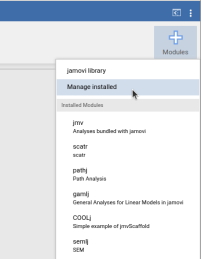
\includegraphics[width=0.4\linewidth]{bookletpics/0_library1} \end{center}

\begin{center}
\includegraphics[width=0.7\linewidth]{bookletpics/0_library2} \end{center}

Installing the module produces a new icon in the icons bar, and the new icon gives access to the list of the module available analyses.

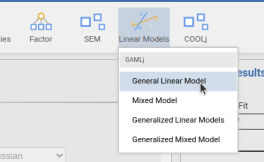
\includegraphics[width=0.5\linewidth]{bookletpics/0_menu1}

Here we always refer to { { GAMLj version ≥ } 3.0.0 }. If you need to work with previous versions, you can refer to GAMLj legacy help
We are ready to go.

\hypertarget{data}{%
\section{Data}\label{data}}

Throughout this book, we are going to use mostly two simulated datasets, containing variables that allow estimating different types of effects for different types of models. Both datasets contain two continuous independent variables, named \texttt{x} and \texttt{z}, two categorical independent variables, named \texttt{cat2} and \texttt{cat3}, with two and three groups respectively. The dependent variable \texttt{y} appears in different forms, or types, so we can apply to it different models. We have a continuous normally distributed dependent variable \texttt{ycont}, a dichotomous version of it \texttt{ybin}, a count version \texttt{ypoi} simulating a Poisson distribution of counts, a ordinal version \texttt{yord} with 5 ordinal levels, and \texttt{ycat}, a three-level categorical variable.

The first dataset containing these variables is called \texttt{manymodels} and simulates a sample of 120 cases drawn randomly for a population. We are going to use this dataset for the general linear model (Chapter \ref{glm}) and the generalized linear models. The second dataset, named \texttt{clustermanymodels} has the same variables, but the data a simulated as drawn from 30 different clusters. We are going to use this dataset for the mixed model and the generalized mixed models.

I agree with the idea that \(x\), \(y\), and \(z\) datasets are boring, and real data examples are more engaging. Nonetheless, \(x\), \(y\), and \(z\) datasets allow exploring many different situations that real data often do not (at least not with one or two datasets), and do not take away the reader's attention from the stats. We will invent some cover story to make the examples more engaging and easier to follow.

Both datasets can be opened from {jamovi} data library.

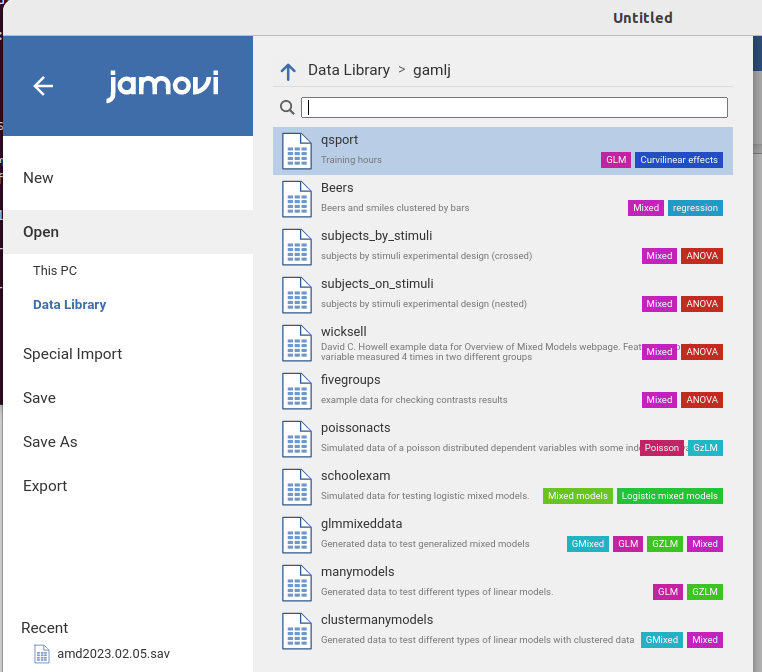
\includegraphics[width=0.7\linewidth]{bookletpics/0_datalibrary1}

\hypertarget{naming}{%
\section{What's in a name}\label{naming}}

All the fundamental analyses presented in this book are referred to as \emph{models}. With the term \emph{model} I mean a concise and efficient way to represent and quantify the relationships among variables. A simple regression, an ANOVA, or a multi-level random coefficients logistic regression are all models of the data. To put it in a more elegant way, a model provides an approximate and idealized representation of the process generating the data \citep{neyman1957inductive}. In several statistical and methodological sources these \emph{models} are called \emph{statistical techniques}, but I do not find this term helpful, because almost everything one does can be a technique. To avoid confusion, we call \emph{models} the linear representation of the dependent variable(s) as a function of the terms of the independent variables. Thus, we have different models when the linear representation is different, or the estimation method is different. A logistic model, for instance, is different from a Poisson model because the first predicts the logit of a dichotomous dependent variable, the second the log of it (more on this later).

In this book we cover four model categories:

\begin{itemize}
\tightlist
\item
  The general linear model (Chapter \ref{glm})
\item
  The generalized linear model (Chapter \ref{gzlm})
\item
  The mixed linear model (Chapter \ref{mixed})
\item
  The generalized mixed model (Chapter \ref{gmixed})
\end{itemize}

The main differences among them, at least the ones we are interested in, can be classified depending on the type of dependent variable they model and the way the sample has been drawn:

Clustered vs independent cases differ in the way the data are collected. We talk about it in Chapter (XX). In general, we will see for each model how and why one of these macro-categories applies.

\hypertarget{angles}{%
\subsection{Statistical techniques vs points of view}\label{angles}}

With a model, we can do many things. First, we evaluate the results. A linear model can always be evaluated from two different angles: The model fit (variances explained or deviance reduced) and the size and direction of the effects (the coefficients). Thus, whenever we estimate a model, we can look at it from each of these angles or both. The model fit, often broken down by variables and effects unique contribution, informs us about the ability of the independent variables to explain the variability of the dependent variable. This angle offers also effect size indices, like \(\eta^2\) or \(\omega^2\). This angle is useful, among other things, to evaluate the strength of the effects. In the linear model, this angle is called \emph{Analysis of Variance}, shorten in \emph{ANOVA}, in the generalized linear model it is called \emph{Analysis of Deviance} (not shorten).

The second angle looks at the coefficients, that represent expected changes in the dependent variable as one compares different levels of the independent variable(s). They answer questions like ``What is the average increase in salary for every year worked?'', or ``what is the group with the largest salary among some employees groups?''. The coefficients angle also provides effect size indices, such as the \(B\) and the \(\beta\) coefficients, the correlation, and several variations of standardized mean differences (Cohen's d). This angle is useful, among other things, to evaluate both the intensity and the direction of the effects.

In {GAMLj}, both points of view are available for all linear models handled by the module, no matter how complex they are. But this creates often confusion in users acquainted with old-fashion terminology. Why is there an ANOVA table in the results section of a regression? Why do I get regression coefficients for categorical independent variables? The reason is that in the linear model's realm, terms such as regression or ANOVA are not \emph{analyses} or \emph{statistical techniques}, they are angles from which one looks at the results. If one is interested in the direction of the effects, one looks at the coefficients, if one is interested in the variability accounted for by the effects, one looks at the variances (or deviance). Thus, what people usually call \emph{ANOVA}, meaning the analysis of a design with one continuous dependent variable and one or more categorical independent variables (factors), is just a general linear model evaluated only from the point of view of the explained variances. What people call \emph{regression} is a general linear model with continuous independent variables for which the analyst focuses on the coefficients. ANCOVA? A general linear model with at least one focal categorical variable and at least one continuous variable, for which the analyst focuses on the effect of the categorical variable knowing that the continuous variable(s) is (are) kept constant. The same applies to any other model, general, generalized, mixed, or generalized mixed.

In this book we keep using terms such as \emph{regression} or \emph{ANOVA}, keeping in mind that we can do well without them.

\hypertarget{statistical-techniques-vs-analyses}{%
\subsection{Statistical techniques vs Analyses}\label{statistical-techniques-vs-analyses}}

Alright, so what do we mean by \emph{statistical techniques} in this book? Things we do with the model. If we find a main effect of a categorical independent variable, we usually want to probe it and check which group is different from any other group. We employ a \emph{posthoc test} technique. Along the way, we also want to see the \emph{estimated marginal means} for each level of the independent variable. If an interaction appears solid in our results, we often probe it to estimate and test the effect of one variable at different levels of another, so we do a \emph{simple effects} technique. In other cases, we want to compare one big model with a smaller one, in which some terms are absent. We do a \emph{model-comparison} technique, so we can evaluate the overall contribution of the effects that are in the big model and not in the smaller (nested) one.

{GAMLj} provides these techniques (and many others) for all models estimable within the module, with the same user interface and results tables. The basic principle that {GAMLj} tries to follow is that \emph{if we can do something in one model, we can do it with any other model}.

\hypertarget{terms-that-we-need-to-generalize}{%
\subsection{Terms that we need to generalize}\label{terms-that-we-need-to-generalize}}

In the methodological literature, statistical techniques emerge often in one field for one application, and then emerge again in other fields or for other applications and get different names. This may create confusion. To clarify, we are going to use some simplification. The most important ones are the following:

\begin{itemize}
\item
  Any \emph{ANOVA like} results, not matter how they are tested (F-test, LRT, \(\chi^2\)), are referred to as \emph{Omnibus tests}.
\item
  \emph{Moderation} is an interaction in which the analyst focuses on one effect and desires to evaluated it at different levels of the other variable involved in the interaction, no matter whether the variable is continuous or categorical. A \emph{moderator} is a variable that the analyst believes can change the effect of an independent variable, no matter the types of variable involved in the analysis.
\item
  Estimating the effect of one variable at different levels of a moderator is called \emph{Simple Effects}, no matter the types of variable involved. So, slicing of an interaction in the (classical) ANOVA or a simple slopes analysis are all refereed to as \emph{Simple Effects} technique (they are indeed the same technique).
\item
  \emph{Estimated marginal means} are the average predicted values of a model for some level of the independent variables. No matter which model we have at hand, and what kind of variables we have, we always mean this.
\end{itemize}

\hypertarget{covnames}{%
\subsection{Terms we need to cope with}\label{covnames}}

In linear models, independent variables are of two kinds: \emph{categorical} or \emph{continuous}. The former defines nominal levels (groups or conditions) the latter defines quantities. Despite the simplicity of this definition, commonly used statistical software calls a categorical independent variable as \emph{factor} and a continuous independent variable as \emph{coviariate}. {jamovi} and {GAMLj} follows this tradition. We should be aware, however, that these terms do not mean anything else that categorical and continuous variables. Every independent variable in a linear model is covariated (partialed out) when the other variable effect is computed, no matter whether the variable is a categorical or continuous one. How it is covariated, however, depends on the model, so we need to pay attention to that.

\hypertarget{general-references}{%
\section{General References}\label{general-references}}

Obviously, I did not invented any of the statistical ideas or methods that this book mentions. Much of this material comes from statistical common knowledge and logical necessity. However, when not otherwise specified, the fundamental concepts treated here can be found in the seminal work of \citet{cohen2014applied}, \citet{searle2016linear}, \citet{raudenbush2002hierarchical}, \citet{agresticategorical}, \citet{aiken1991multiple}. When needed, specific references are provided for more novel or critical issues.

\hypertarget{glm}{%
\chapter{The General Linear Model}\label{glm}}

{ Draft version, mistakes may be around }

\hypertarget{introduction}{%
\section{Introduction}\label{introduction}}

The general linear model (GLM) encompasses a wide range of analyses that are commonly used in statistical practice. It holds significant importance as having a good understanding of the GLM can be highly beneficial. Within the realm of GLM, various analyses such as simple and multiple regression, Pearson correlation, independent-samples t-test, ANOVA, ANCOVA, and related derivations like mediation analysis, planned comparisons, etc., can be found (cf.~Section \ref{naming}). These applications share a common theme: the dependent variable is continuous, ideally following a normal distribution, and the sample consists of non-related, independent cases. Among these applications, one of the fundamental yet crucial model is the simple regression, which is a GLM with a single continuous independent variable (IV).

\hypertarget{regression}{%
\section{One continuous IV}\label{regression}}

\begin{flushright} AKA: Simple Regression  \end{flushright}

Consider the dataset \texttt{manymodels} (cf.~Section \ref{data}). The dependent variable is a continuous variable named \texttt{ycont}, and we want to estimate its linear relation with a continuous variable named \texttt{x}. The extensive representation of the relation between the two variables can be obtained with a scatterplot. It is clear that \texttt{ycont} and \texttt{x} can be any variable, as long as we can consider them as continuous. For the sake of the argument, let us imagine that we went to a bar and measured \texttt{ycont} as the average number of smiles smiled by each customer in a given time and \(x\) as the number of beers drunk for the same period.

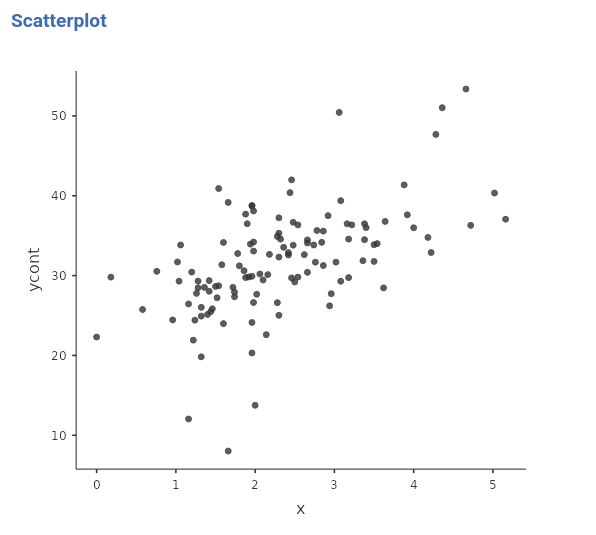
\includegraphics[width=0.8\linewidth]{bookletpics/2_scatterplot1}

What we want to know is the average increase (or decrease) of the dependent variable as the independent variable increases. Thus, how many smiles on average one should expect for one more beer? We ran a GLM to get the answer.

\hypertarget{glminput}{%
\subsection{Input}\label{glminput}}

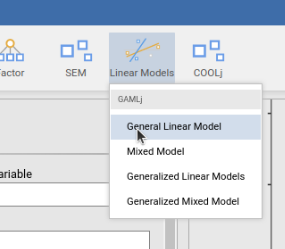
\includegraphics[width=0.5\linewidth]{bookletpics/2_menu1}

We set the \texttt{ycont} variable as the dependent variable and the \texttt{x} variable as the independent continuous variable (see \ref{covnames}), and look at the results.

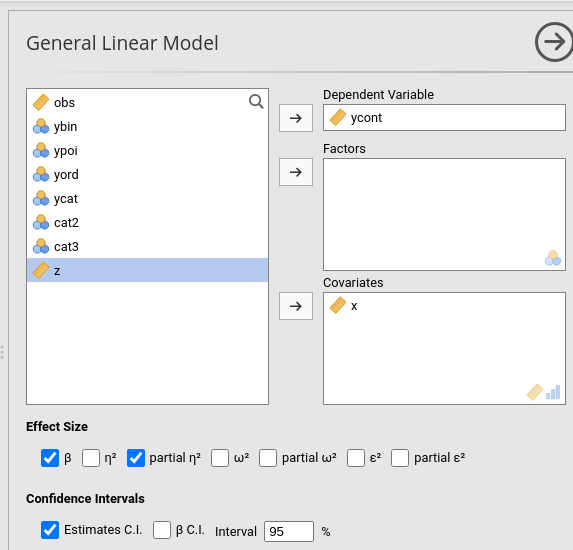
\includegraphics[width=0.7\linewidth]{bookletpics/2_input1}

\hypertarget{model-recap}{%
\subsection{Model Recap}\label{model-recap}}

First, we check out the {Model Info} Table.

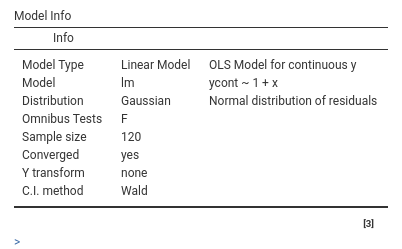
\includegraphics[width=0.7\linewidth]{bookletpics/2_output1}

This is a recap table that says that we did what we wanted to do, and how we did it. The second table we get is the {Model Fit} Table, where the \(R^2\), the adjusted \(R^2\), and their inferential test are presented.

\hypertarget{twofit}{%
\subsection{Model Fit}\label{twofit}}

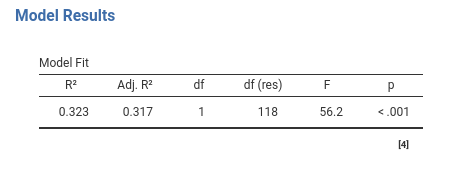
\includegraphics[width=0.7\linewidth]{bookletpics/2_output2}

The \(R^2\) gives us the first glance of the model from the \emph{variance angle} (cf.~Section \ref{angles}). The short story says that our model (in this case the independent variable \(x\)) explains, or accounts for, 32.3\% percent of the variance. So, if all differences in the smiles (\texttt{ycont}) are set to 100, 32\% of them can be associated with the number of beers drunk (\(x\)). The \texttt{Adj.}\(R^2\) is the estimation of the variance explained by the model in the population, and the \texttt{df} is the number of parameters estimated by the model apart from the intercept: Here is one because we have one independent variable that requires only one coefficient. The \texttt{F} column gives the F-test testing the null hypothesis that \(R^2\) is zero, and \texttt{p} is the probability of obtaining the observed \(R^2\) under the null hypothesis. If you find this story a bit dull, you might want to read the full story in Appendix \ref{appendixa}.

\hypertarget{omnibus-tests}{%
\subsection{Omnibus Tests}\label{omnibus-tests}}

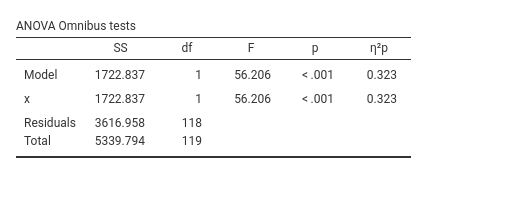
\includegraphics[width=0.8\linewidth]{bookletpics/2_output3}

With only one continuous variable this table is not very useful, but we comment on it anyway to get us familiar with the ideas of the two points of view always available in a linear model (cf \ref{angles}). The first line, included for legacy compatibility reasons, presents the inferential test for the model as a whole, which we have already encountered in Section \ref{twofit}. The second line provides information about the amount of variance in the dependent variable that can be explained by the independent variable. In this case, the \(p\eta^2\) is equal to the \(R^2\), because there is nothing to partial out (there is only one independent variable). Instructive, however, is to select the option \(\epsilon^2\).

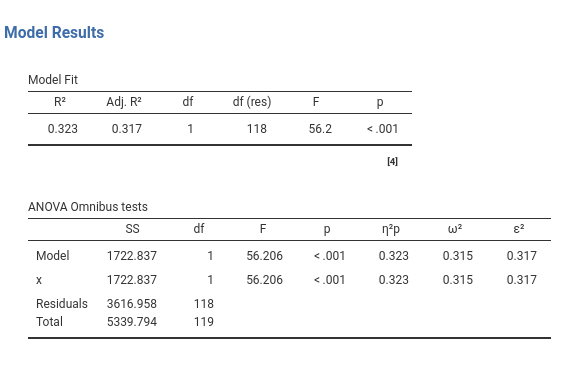
\includegraphics[width=0.9\linewidth]{bookletpics/2_output4}

we can notice that the \(\epsilon^2\) is equal to the adjusted \(R^2\). Yes, that is going to stay:

\(R^2\) and \(\eta^2\) indices (partial or not) are the sample estimates of variance explained, whereas \(R_{adj}^2\) and \(\epsilon^2\) effect size indices (partial or not) are the population version (\(\omega^2\) is population too). People tend to use the sample version of these indices (\(\eta^2\) and \(R^2\)) when they should use the population version (\(R^2_{adj}\) and \(\epsilon^2\)). The same goes for \(\omega^2\) index, but you want to read this about why you want to use them, and this how they are computed . In a nutshell, \(R^2\) and \(\eta^2\) tell what happened in the sample, \(R_{adj}^2\) and \(\epsilon^2\) tell what should happen in the population.

\hypertarget{glmcoefs}{%
\subsection{Coefficients}\label{glmcoefs}}

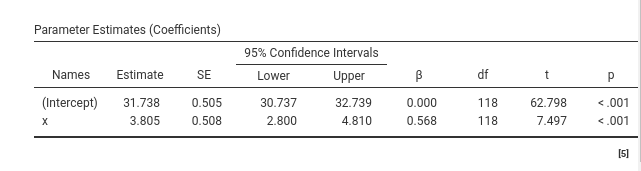
\includegraphics[width=0.9\linewidth]{bookletpics/2_output5}

The regression coefficients table, here called the {Parameters Estimates (Coefficients)} table, informs us about the size and the direction of the effect. The interesting coefficient is the one associated with the independent variable (the \texttt{Estimate} column). Here it is \(3.808\). This means that for every unit increase in the independent variable the dependent variable increases, on average, of \(3.808\) units. In our toy example, for each beer one drinks, on average, one smiles \(3.808\) smiles more. This is the \textbf{regression coefficient}, the very first and most solid pillar of the linear model. This interpretation is going to stick, so keep it in mind, because when models get more complex, we are going to amend it, but only to make it more precise, never to betray it.

The intercept, which is not focal here (\emph{nobody looks at the intercept}), is worth mentioning for the sake of comparison with other software. If you run the same analysis in SPSS, R, Jasp, Stata, etc, you get the same \texttt{estimate} for the \texttt{x} variable, but a different \texttt{(Intercept)}. Recall that in any linear model the intercept is the expected value of the dependent variable for \(x=0\). In {GAMLj}, however, the independent variables are centered to their means by default, so \(x=0\) means \(x=\bar{x}\). So, in {GAMLj} the intercept is the expected value of the dependent variable for the average value of \(x\).

Why centering? First, centering does not change the results of the regression coefficients of simple and multiple regression, so it is harmless in many situations. However, when an interaction is in the model, centering guarantees that the linear effects are the \emph{main effects} one expects, and not some weird effects computed for the moderator equal to (possibly non-existing) zero. Furthermore, I believe that very few variables have a real and meaningful zero, so their mean is a more sensible value than zero \footnote{I have nothing against zero: my favorite number is 610, which in Italian literally translates to \emph{you are a zero}, where ``you'' is meant to be ``we all''}. If your variables really have a meaningful zero (which you care about), you can always ``unscale'' your independent variables setting them to \texttt{Original} in the {Covariates scaling} panel.

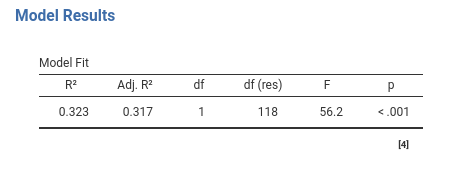
\includegraphics[width=0.8\linewidth]{bookletpics/2_output2}

\hypertarget{pearson-correlation}{%
\subsection{Pearson Correlation}\label{pearson-correlation}}

Across sciences, the most used index of association between two variables is the Pearson Correlation, \(r\), otherwise named zero-order correlation, bivariate correlation, standardized covariance index, product-moment correlation, etc (pick any name, the Pearson correlation is a case of the Stigler law of eponymy anyway).

What is important here is that the Pearson correlation is just the standardized regression coefficient of a GLM with only two continuous variables (one {DV {Dependent Variable} }, on {IV {Independent Variable} }). In GLM terminology, it takes the name of \(\beta\). In our example, the correlation
between \texttt{ycont} and \texttt{x} is \(.568\). We can verify this by asking {jamovi} to produce the correlation between the two variables in the {Regression-\textgreater Correlation Matrix} menu.

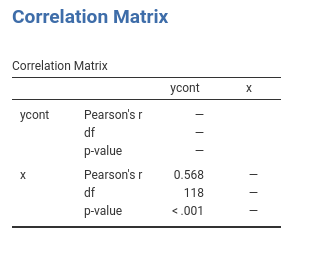
\includegraphics[width=0.5\linewidth]{bookletpics/2_output8}

As expected, the correlation and the \(\beta\) are the same. More specifically, the Pearson correlation is the regression coefficient that one obtains if the GLM is run after standardizing (computing the z-scores) both the dependent and the independent variable. This gives us a key to interpret the Pearson correlation in a precise way: Remembering that any standardized variable has 0 mean and standard deviation equal to 1, we can interpret the \(r\) (and therefore the \(\beta\)) as the number of standard deviations the dependent variable moves as we move the independent variable of one standard deviation. It varies from -1 to 1, with 0 meaning no relation.

When we deal with GLM with more than one independent variable, the link between the \(\beta\) and the Pearson correlation is lost, but \(\beta\)'s remain the coefficients obtained after standardizing the variables, so they remain the standardized coefficients.

If the user decides to report the \(\beta\) coefficients, they would likely want to report the \(\beta\) confidence intervals. They can be asked for in the input by flagging the ``\(\beta\) C.I. option''.

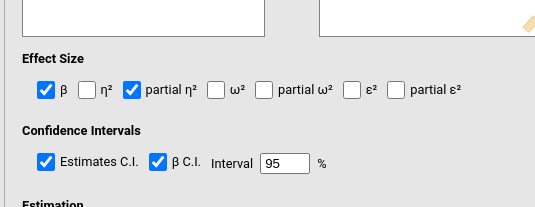
\includegraphics[width=0.6\linewidth]{bookletpics/2_simple_input9}

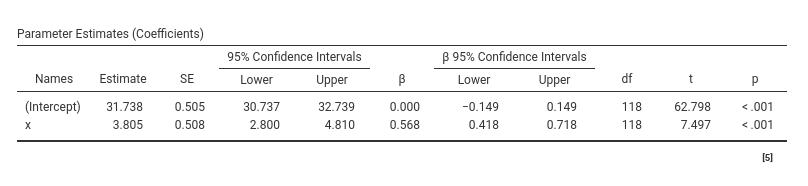
\includegraphics[width=0.9\linewidth]{bookletpics/2_simple_output9}

\hypertarget{glmplot}{%
\subsection{Plots}\label{glmplot}}

It is always a good idea to look at your model results with a plot. A plot shows your fitted model (predicted values). Because a model is always an approximation of the real data, we want to show our predicted values against, or together, the actual data. In {Plots} panel, we can set up a plot as follows:

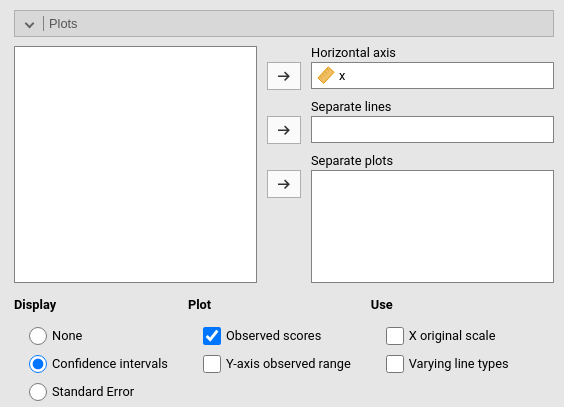
\includegraphics[width=0.7\linewidth]{bookletpics/2_input3}

and see the results:

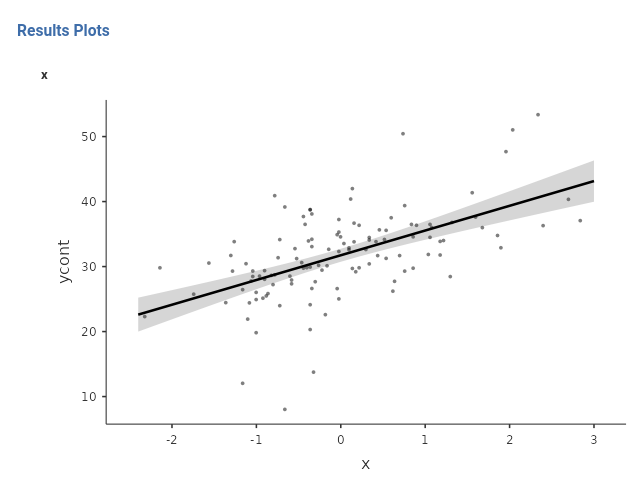
\includegraphics[width=0.8\linewidth]{bookletpics/2_plot1}

By default, the plot shows also the confidence bands around the regression line. The bands are the continuous version of the confidence intervals, and indicate the range of values where the predicted value are expected to lay.

Notice that the independent variable scale is centered to 0. This is because {GAMLj} centers continuous variable by default (cf \ref{glmcoefs}). If a plot with the original scale is preferred, one can flag the option {X original scale} in the {Plots} panel.

\hypertarget{multiregression}{%
\section{More continuous IVs}\label{multiregression}}

\begin{flushright} AKA: Multiple Regression  \end{flushright}

Let us add to our model the \texttt{z} variable, again a continuous variable. To keep up with our toy example, let's assume that \texttt{z} was a measure of participants' extroversion.

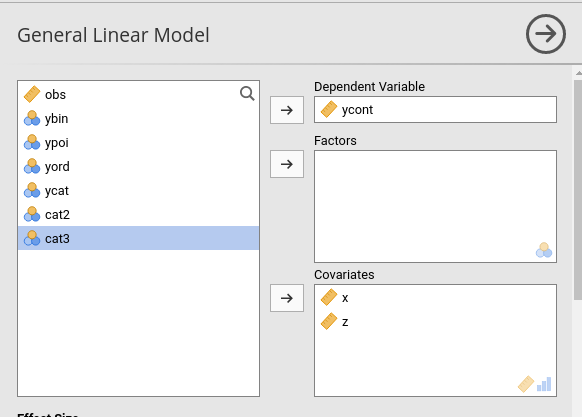
\includegraphics[width=0.7\linewidth]{bookletpics/2_input4}

The results are now updated. Let's go through the most important tables.

\hypertarget{twofit2}{%
\subsection{Model Fit}\label{twofit2}}

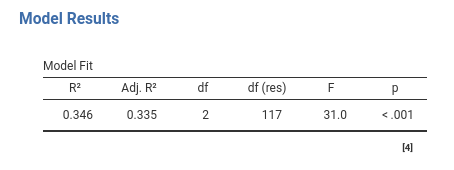
\includegraphics[width=0.7\linewidth]{bookletpics/2_output6}

The \(R^2\) gives us the variance explained, or accounted for, of the dependent variable by the whole model. This means by both \texttt{x} and \texttt{z}, alone and together. The overall variance explained is statistically different from zero, so we can say we do explain some variance of \emph{smiles} (\texttt{ycont}) thanks to the variability of \emph{beers} (\texttt{x}) and \emph{extroversion} (\texttt{z}). The issue is now how to quantify each independent variable contribution to this variance explained. We need to look at the individual contributions, so the {Omnibus Tests}.

\hypertarget{variances}{%
\subsection{Omnibus Tests}\label{variances}}

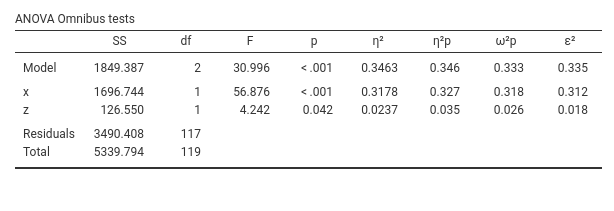
\includegraphics[width=0.9\linewidth]{bookletpics/2_output7}

Please notice that I selected \(\eta^2\), \texttt{partial} \(\eta^2\), \(\epsilon^2\), and \texttt{partial} \(\epsilon^2\), so we can interpret these indices. Before that, however, we can mention that the \texttt{x} variable effect is statistically different from zero, F(1,117)=58.87, p.\textless.001, whereas the effect of \texttt{z} reaches the predefined level of significance by a very tiny margin, F(1,117)=4.242, p.=.042. So we can say that there is enough evidence to believe that both effects are different from zero, although the former seems more solid than the latter. Statistical significance, however, is only a part of the story: effects should be evaluated on at least three dimensions: \textbf{significance}, \textbf{size}
and \textbf{direction}. We now want to evaluate their size.

Effect size indexes are good tools to evaluate effect sizes (\emph{nomen omen}). We start with the \texttt{partial} \(\eta^2\), mainly because it is the most used and reported one effect size index in the literature (I always thought that is the case because it is the only ES produced by SPSS GLM). The \texttt{partial} \(\eta^2\) is the proportion of variance uniquely accounted for by the independent variable, expressed as the proportion of the variance of the dependent variable not explained by the other independent variables. In short, for \texttt{x} (\emph{beers}) is the proportion of variance of \emph{smiles} not explained by \emph{extroversion} that is explained by \emph{beers}. In other words, it answers the question: if everybody had the same level of \emph{extroversion}, how much variance would \emph{beers} explain?

Please note that the unique variance explained by the variable beers (\(x\)), which amounts to 31.2\%, is calculated after removing the variance accounted for by the variable extroversion (\(z\)). Frequently, one is interested in determining how much variance a variable explains in relation to the total variance of the dependent variable. This is referred to as \(\eta^2\), which represents the variance uniquely explained by a variable as a proportion of the total variance in the dependent variable. In other words, it answers the question: how much of the variance in smiles would be uniquely explained by beers?

The \(\epsilon^2\) and \texttt{partial} \(\epsilon^2\) indexes can be interpreted as the \(\eta\)'s, but they are adjusted to represent the population variances, not the sample variances. So, they are better estimations of the ``real'' effect size indexes.

A detailed description of the computation of these indexes can be found in GAMLj help page

\hypertarget{household-chores}{%
\subsection{Household Chores}\label{household-chores}}

Assuming you live in a house with another person, there are a total of 100 chores to be done in your household, such as washing the dishes, cleaning the windows, and taking the dog out for a walk. Out of these chores, you personally handle 20 of them, with 5 being done together with your companion. On the other hand, your companion takes care of 40 chores (they always do a better job), including the ones that you both do together. Therefore, collectively, you and your companion complete 55 chores, while your companion handles 35 chores alone and you handle 15 chores alone. Additionally, there are 5 chores that are done together.''

As a couple, your overall contribution is 55/100, so your \(R^2=.55\). You alone did 15 chores, so your unique contribution is \(\eta^2=15/100=.15\) of the total amount of chores to be done. However, of the chores left to do by your companion (60), you did alone 15, so your \emph{partial} contribution is \(p\eta^2=15/60=.25\).

The distinction between \(\eta^2\) (or any non-partial effect size) and its partial version lies in the denominator used. Non-partial effect size indexes represent proportions of the total variance, while partial effect size indexes represent proportions of the total variance minus the portion accounted for by other variables.

In any household, we would use the \(\eta^2\), but many authors are still using the \(p\eta^2\). What is important is to know the difference between the two computation methods, so we can feel free to use which one we prefer. A deep discussion of this matter can be found in \citet{olejnik2003generalized}, which I recommend reading.

\hypertarget{coefficients}{%
\subsection{Coefficients}\label{coefficients}}

Now we look at the direction and intensity of the effects, interpreting the {Parameters Estimates (Coefficients)} Table.

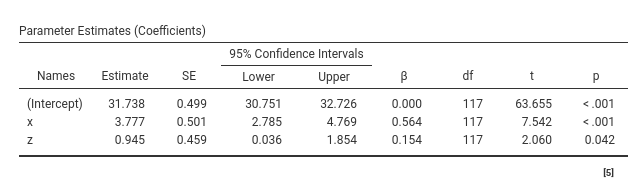
\includegraphics[width=0.9\linewidth]{bookletpics/2_output9}

For each variable effect, we see the \texttt{Estimate} (usually called the \(B\) coefficients), the standard error (\texttt{SE}), the confidence interval, the \(\beta\), the degrees of freedom (\texttt{df}), the t-test (\texttt{t}) and the p-value (\texttt{p}). So, the full set of estimates (\(B\) and \(\beta\)) and the inferential tests (t-test, C.I. df and p-values). Let's interpret them for \(x\):

\begin{itemize}
\tightlist
\item
  \(B\) : keeping constant \(z\), for one unit more in \(x\) we expect the dependent variable average score to increase of \(3.777\) units.
\item
  \(\beta\) : the effect corresponds to a standardized coefficient of \(.564\), indicating that for one standard deviation more in \(x\), \(ycont\) increases of .564 standard deviations, keeping constant the effect of \texttt{z}.
\item
  \(C.I.\) : ``Were this procedure to be repeated on numerous samples, the proportion of calculated 95\% confidence intervals that encompassed the true value of the population parameter would tend toward 95\%'' (cf.~Wikipedia). Weird? Yes, that's what confidence intervals are. But what about 2.785 and 4.769? Well, The two values, known as confidence bounds, encompass 95\% of the cases in the distribution of sample estimates if, and only if, we have accurately captured the true population parameter in our sample. However, since we cannot assess whether we have indeed done so, this interpretation is not justified. Nevertheless, if we state that we expect the population parameter to fall within this range and continue making such statements indefinitely, we will be correct approximately 95\% of the time. From a practical point of view, we can use the confidence interval width as an indicator of accuracy and precision of our estimate. If one tells us that our chances of winning a bet lay between 10\% and 90\%, we will consider this hint much less precise that if we are told that they vary from 45\% to 55\%.
\end{itemize}

While this book does not delve into the intricacies of confidence intervals, interested readers may find \citet{mayoci}'s work on the subject enjoyable to read.

\hypertarget{moderation}{%
\section{Continuous IVs and interaction}\label{moderation}}

In the previous model, we can make a plot of the effect of beers (\texttt{x}) on smiles (\texttt{ycont}), at different levels of extroversion (\texttt{z}). This can be achieved in {GAMLj} by asking for a plot as follows:

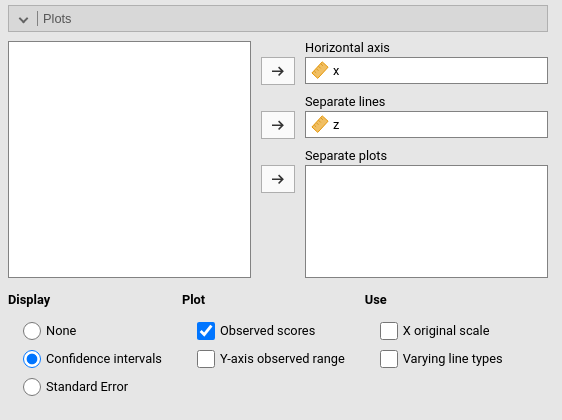
\includegraphics[width=0.7\linewidth]{bookletpics/2_input10}

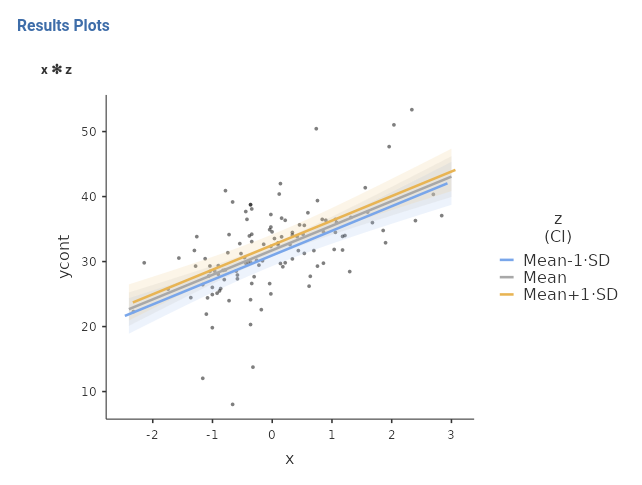
\includegraphics[width=0.9\linewidth]{bookletpics/2_output10}

The three lines depicted in the plot are the effects of \texttt{x} on \texttt{ycont}, estimated at different levels of \texttt{z}. Because \texttt{z} is continuous, {GAMLj} automatically sets the focal levels of \texttt{z} equal to the mean, one SD above the mean, and one SD below the mean (this can be changed, see below).

As expected, the three effects depicted are perfectly parallel. This is because in multiple regression, the effect of each variable is computed keeping constant the other variable, which is equivalent to saying that the effect is computed as if it were the same at each level of the other variable. In other words, the effects at different levels of the other variable are forced to be the same, no matter the data. But this constrain can be removed by adding an interaction in the model.

An interaction allows the effect of one variable to vary at different levels of another variable. Essentially, an interaction signifies that the effect of variable \(x\) depends on the levels of variable \(z\). The interaction coefficient quantifies the extent of change in the effect of one variable across various levels of the other. Specifically, the interaction coefficient represents the expected change in the effect of one independent variable when the other independent variable increases by one unit.

Let's do it. In the {Model} panel, we select both variables on the left field and move them together to the right field, defining an interaction \(x*z\).

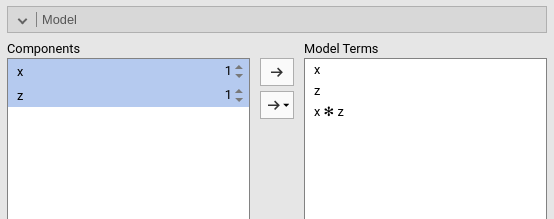
\includegraphics[width=0.7\linewidth]{bookletpics/2_input11}

The results updated accordingly showing also the interaction effect.

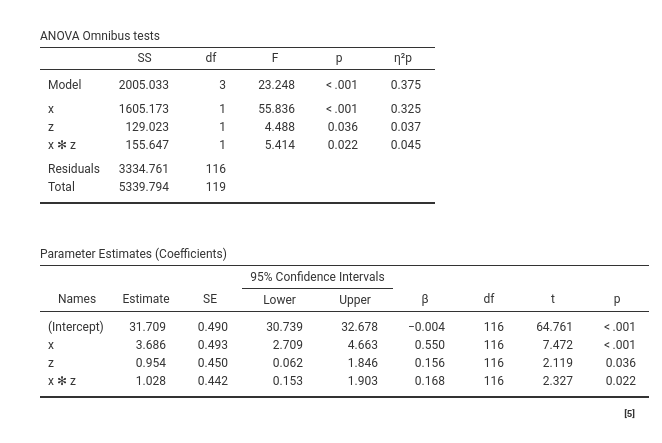
\includegraphics[width=0.9\linewidth]{bookletpics/2_output11}

Let's focus on the {Parameter Estimates (Coefficients)} Table. When there is an interaction in a linear model, the effect associated with the independent variables are the effect of the independent variable computed for the other variable equal to zero. This is not a software choice, that is the way a linear model is \citep{aiken1991multiple}. However, {GAMLj}, by default, centers the continuous variables to their means, so the linear effects can be interpreted as \emph{main effects}, namely, the effect of the variable computed on average, at the average level of the other variable. Thus, we can say that, \emph{on average}, beers (\(x\)) has a positive effect on smiles (\(ycont\)) of \(3.686\), corresponding to a standardized effect of \(.550\). For the average level of beers (\(x\)), the effect of extroversion (\(z\)) is \(.954\), corresponding to a standardized effect of \(.156\).

The interaction effect, denoted as \(x*z\), indicates that the effect of beers (\(x\)) increases by 1.028 units for each additional unit of extroversion (\(z\)). This interaction effect is statistically significant, suggesting that the effect of beers varies across different levels of extroversion. It is important to note that the same interpretation holds true if we reverse the roles of \(x\) and \(z\). In other words, the effect of extroversion (\(z\)) differs at various levels of beers (\(x\)).

\hypertarget{modint}{%
\section{Moderation=interaction}\label{modint}}

Many authors calls this type of effect a moderation effect. They are correct, but there is nothing special about interactions between continuous variables. Any interaction effect, no matter if the independent variables are continuous or categorical, tests a moderation model. The only difference between moderation and interaction is theoretical. When we lay out a theoretical model, we declare which variable is the hypothesized moderator and which is the independent variable. Statistically, they are equivalent, and the strength of moderation is tested with an interaction. We will see that moderation models are tested also with categorical variables (within what people calls \emph{ANOVA}) or when one variable is categorical and the other is continuous (within what people used to call \emph{ANCOVA}, but not anymore). We have seen that naming techniques rather than models is cumbersome (cf.~Section \ref{naming}). The same goes for \emph{moderation}. Just keep in mind that moderation refers to a theoretical model, its statistical counterpart is the \emph{interaction}, for all kinds of variables.

\hypertarget{simpleslopes}{%
\section{Simple Slopes}\label{simpleslopes}}

When an interaction is present (let's say it is significantly different from zero), we can probe it \citep{aiken1991multiple}. Probing means to estimate, test, and visualize the effect of one independent variable at different levels of the other. The ``other variable'' is usually called the \emph{moderator}: The variable that is supposed to change the effect of the independent variable. In our example, we focus on the effect of beers (\(x\)), and different levels of the moderator extroversion (\(z\)). First, let's look at the plot.

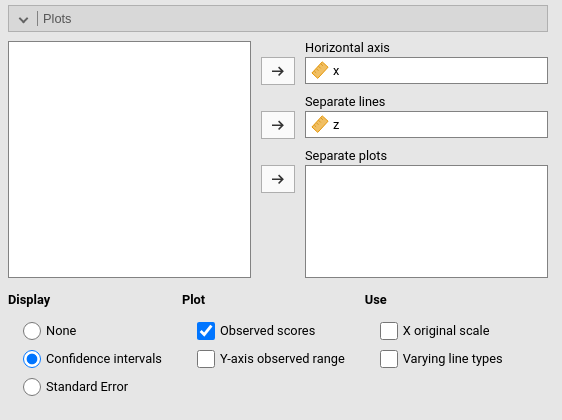
\includegraphics[width=0.7\linewidth]{bookletpics/2_input10}

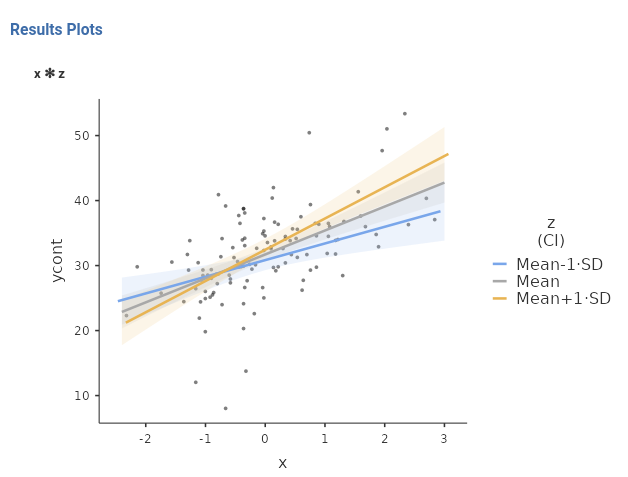
\includegraphics[width=0.9\linewidth]{bookletpics/2_output12}

We can see now that the lines representing the effect of \(x\) at different levels of \(z\) are no longer parallel, they have \emph{different slopes}. Looking at the plot, we can see that the effect of \(x\) is stronger for high levels of \(z\) (\texttt{Mean+1*SD}), than for the average level of \(z\) (\texttt{Mean}) than for low levels of \(z\) (\texttt{Mean-1*SD}).

The plot is very useful to visualize how the effect of one variable changes at different levels of the moderator. Often, however, we also want to estimate those slopes and maybe test them. We can do that in the {Simple Effects} panel. Recall that \emph{simple slopes} is just a name for \emph{simple effects} applied to continuous variables, so {GAMLj} uses the term \emph{simple effects} because it generalizes to any type of independent variable.

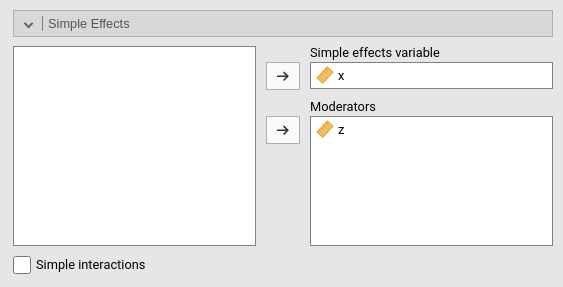
\includegraphics[width=0.7\linewidth]{bookletpics/2_input13}

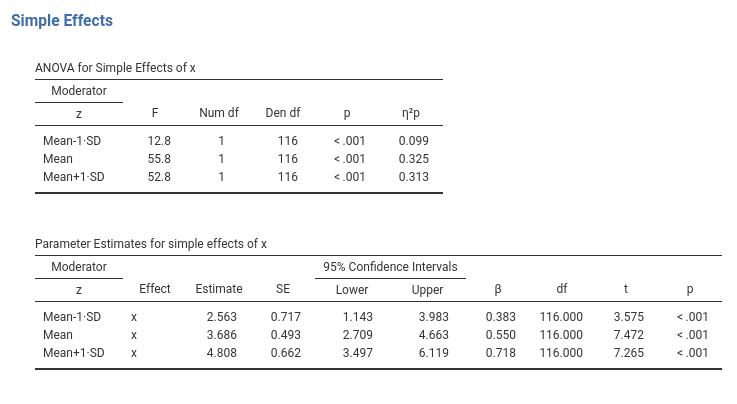
\includegraphics[width=0.9\linewidth]{bookletpics/2_output13}

The first table reports the F-tests and indices of explained variance (\ref{variances}). The coefficients table reports the slopes of the effect of the \texttt{x} variable at different levels of the \texttt{z} variable. Practically, the tables report the effect sizes and the inferential tests associated with the lines depicted in the plot.

If one wants to change the levels of the moderator at which the effects are estimated and plotted, one can go to the {Covariate Scaling} panel and change the \texttt{Covariate\ conditioning} setup. For instance, one may want to explore the effect of \texttt{x} at 2 SD away from the mean, so one sets the field under Mean \(\pm\) SD to 2. One can also decide to condition the slopes to specific percentiles of the \texttt{z} variable, by selecting Percentiles \(\pm\) SD, which conditions to 25th, 50th, 75th percentile (cf GAMLj help page).

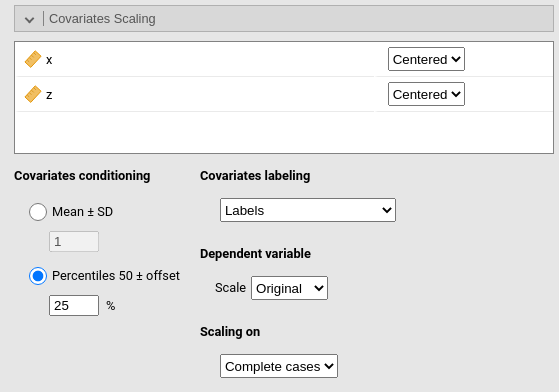
\includegraphics[width=0.7\linewidth]{bookletpics/2_input14}

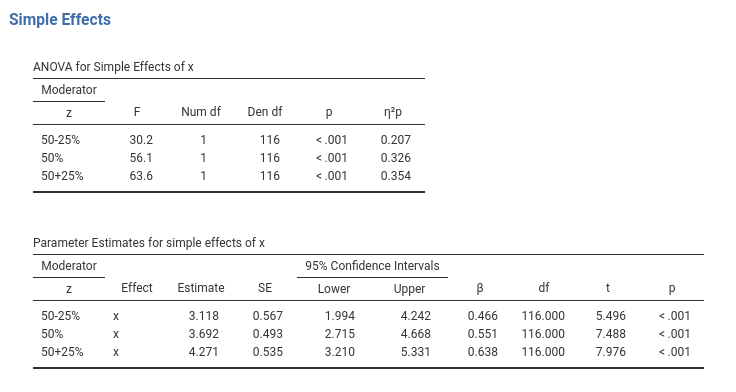
\includegraphics[width=0.9\linewidth]{bookletpics/2_output14}

We can be happy with the analysis, as we have estimated, tested, and quantified all the interesting effects of our independent variables on the dependent variables. We discuss simple effects again in \ref{simpleinteractions}. An equivalent example, with different data, can be found in GAMLj help page: GLM example 1.

\hypertarget{anova}{%
\section{Categorical IVs}\label{anova}}

\begin{flushright} AKA: ANOVA  \end{flushright}

We can now work with a model with categorical independent variables. The dataset provides \texttt{cat2} and \texttt{cat3} variables, with two groups and three groups respectively. Their combination produces the following groups.

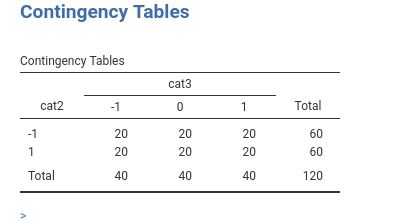
\includegraphics[width=0.7\linewidth]{bookletpics/2_anova_output1}

To put some flesh on the bones, let's imagine that cat3 be the type of beer one drinks, with levels \emph{stout}, \emph{IPA} and \emph{pilsner}. Assume \texttt{cat2} be type of bar, \emph{music bar} vs \emph{sports bar}. To remember, let's put some labels on the variables levels.

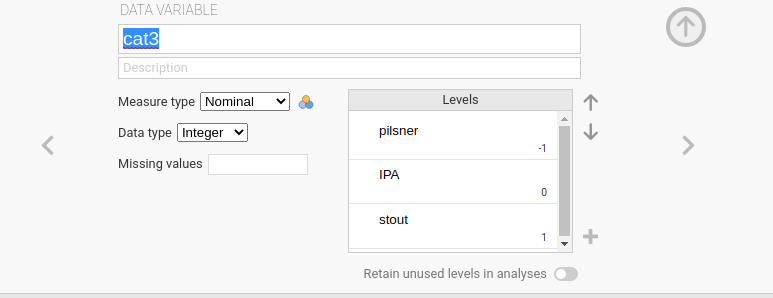
\includegraphics{bookletpics/2_anova_input1.png}
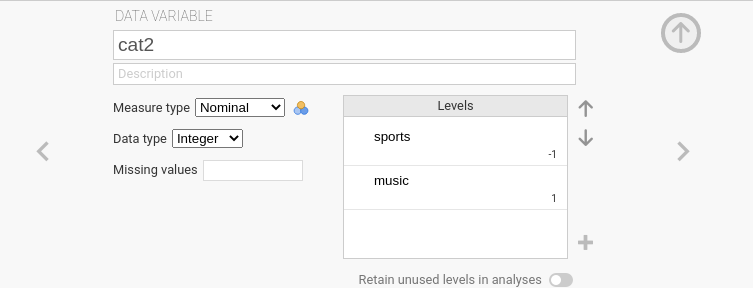
\includegraphics{bookletpics/2_anova_input2.png}

Take a note about the fact that the specific values present in the dataset of a categorical variable have no bearing on the results of the analysis. The categorical variables are coded by {GAMLj} independently of their values: It applies a coding system to cast the categorical {IV {Independent Variable} } into the model. We can also change the coding system with the module options (see below).

We can now run a new model, with \texttt{ycont} as dependent variable, and the two categorical variables as the independent ones.

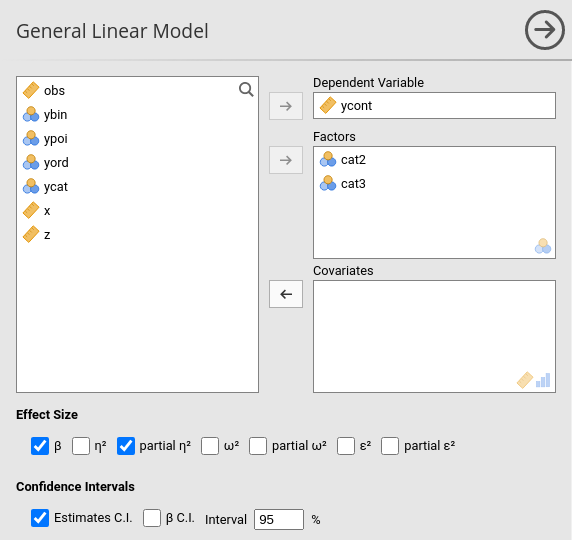
\includegraphics{bookletpics/2_anova_input3.png}

The tables we have seen for the first model are the same produced now, we only need to adjust some interpretation to reflect the categorical nature of the variables.

\hypertarget{model-fit-and-omnibus-tests}{%
\subsection{Model Fit and Omnibus tests}\label{model-fit-and-omnibus-tests}}

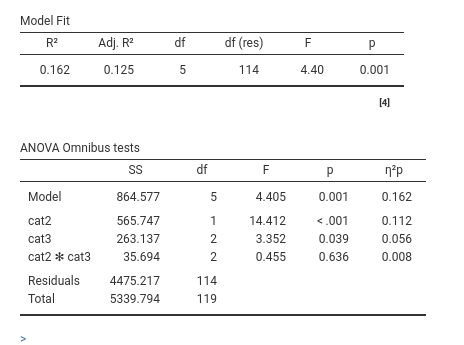
\includegraphics{bookletpics/2_anova_output2.png}

{Model Fit} and {ANOVA Omnibus tests} tables do not require adjustments of the interpretation. Here we see that our model explains \(.162*100\) percent (\(R^2\)) of the dependent variable variance, \(.125*100\) percent as population estimate (Adj. \(R^2\)), and that the type of bar (\texttt{cat2}) has a main effect, type of beer (\texttt{cat3}) has a main effect, and there is no indication of an interaction. Effects are small, with \texttt{cat2} main effect explaing \(.112*100\) percent of the variance not explained by the other effects, \texttt{cat3} main effect explaining \(.056*100\) percent, and the interaction explaining only around 2\% of the partial variance.

\hypertarget{dummies}{%
\subsection{Coefficients}\label{dummies}}

When dealing with categorical independent variables, one usually does not look at the coefficients, but one goes straight to the plots to interpret the results. Nonetheless, the coefficients are present and they can be interpreted.

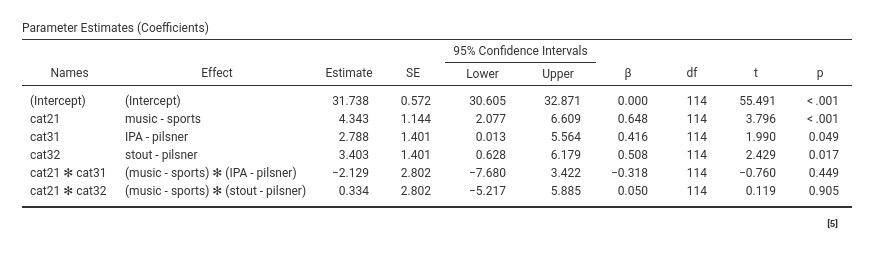
\includegraphics{bookletpics/2_anova_output3.png}

Their interpretation depends on the way the levels (groups) of the variables are coded. In fact, to cast a categorical variable into a linear model (any linear model), it must be coded with weights (numbers) that represent specific contrasts. We need \(K-1\) contrasts to represent \(K\) groups (see appendix \ref{a1dummies} for more details). These contrasts are commonly called \emph{dummy variables}, but it is more correct to call them \emph{contrast variables}. {GAMLj} default uses the \emph{simple} coding system, as it is evident in the {Factor Coding} tab.

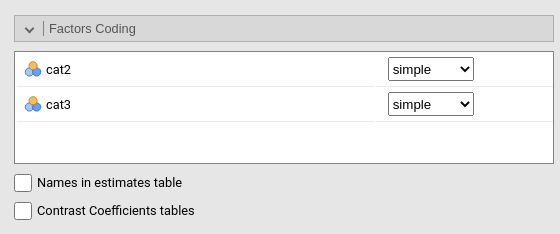
\includegraphics{bookletpics/2_anova_input4.png}

\emph{Simple} coding contrasts estimate the mean difference between one reference group and each of the other groups. The first level present in the dataset is used as reference group. \emph{Simple} coding yields the same comparisons as the more classical \emph{dummy} system, but \emph{simple} coding centers the contrasts to zero, so in the presence of an interaction in the model, the main effects are correctly estimated as \emph{average effects}. So, for \texttt{cat2}, we need only one \emph{contrast} which compares \emph{music} vs \emph{sports}. The coefficient \(4.343\) is the mean difference (in the dep variable) between the two groups. So, people in the \emph{music} bar smile 4.343 smiles more than people in the \emph{sports} bar. For type of beer (\texttt{cat3}), we need two contrast variables, because we have three groups: \texttt{cat31} compares the reference group \emph{pilsner} against \emph{IPA}, the second contrast \texttt{cat32} compares \emph{pilsner} with \emph{stout}. The remaining coefficients are required to estimate the interaction \texttt{cat2\ X\ cat3}.

We should notice that the model does not estimate all possible contrasts, for instance \emph{stout} is not compared with \emph{IPA}. The reason is that those contrasts are redundant in order to capture the whole explained variance (cf.~Appendix \ref{a1dummies}). If one needs all possible comparisons, one can use {Post Hoc Tests} panel to obtain the comparisons (cf.~\ref{posthoc}).

{GAMLj} offers several coding systems to code the categorical variables. If you want to take a look at what the contrasts are comparing, you can ask for {Contrast Coefficients tables}, so a table visualizing the actual coding is produced.

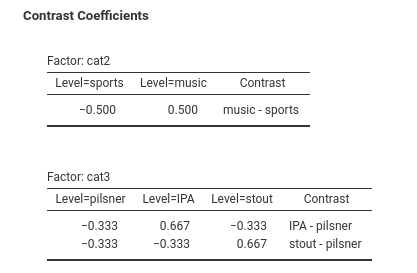
\includegraphics{bookletpics/2_anova_output4.png}

All coding system used in {GAMLj} are explained in details in the GAMLj help page: contrasts.

\hypertarget{plots}{%
\subsection{Plots}\label{plots}}

As for the continuous {IVs {Independent Variables} } case, we can plot the results. When the {IVs {Independent Variables} } are categorical, we obtain the plot of the means.

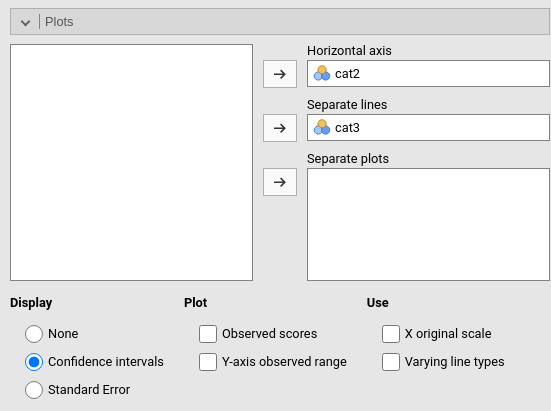
\includegraphics{bookletpics/2_anova_input5.png}
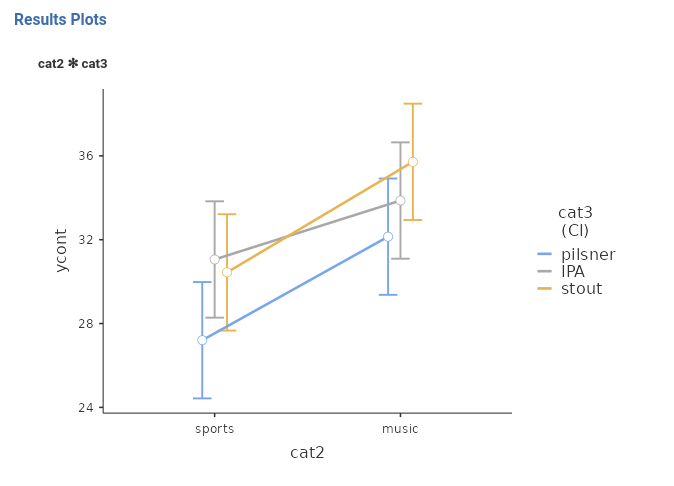
\includegraphics{bookletpics/2_anova_output5.png}

From the results is evident the main effect of \texttt{cat2}, with \emph{music} bar showing a higher average than \emph{sports} bar, and a small main effect of type of beer, with \emph{stout} vaguely larger than \emph{IPA} and larger than \emph{pilsner}.

\hypertarget{posthoc}{%
\section{Post-hoc tests}\label{posthoc}}

Sometimes people want to probe main effects or interactions of categorical variables to test all possible comparisons among means. It should not be a habit to do so, because the coefficients table already provides comparisons that may be enough to explain the results. One can also use a simple effects analysis to test specific comparisons. Nonetheless, if one really needs all possible comparisons, one can use the {Post Hoc Tests} panel. Here we ask for the \emph{post hoc} tests of the variable \texttt{cat3}, because \texttt{cat2} features only two levels, so probing is useless (we have already its main effect). In this example we do not probe the interaction, because it is very small and not significant, but the module allows probing all possible effects.

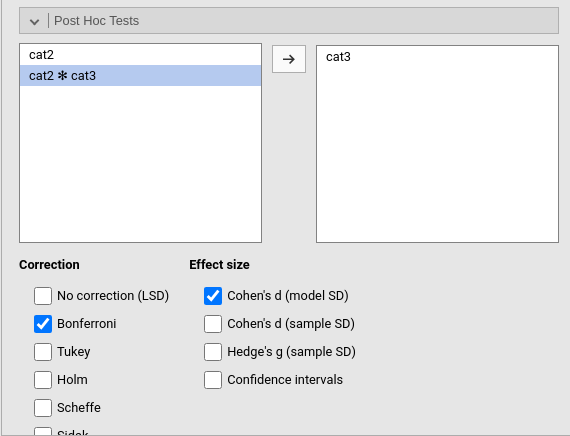
\includegraphics{bookletpics/2_anova_input6.png}
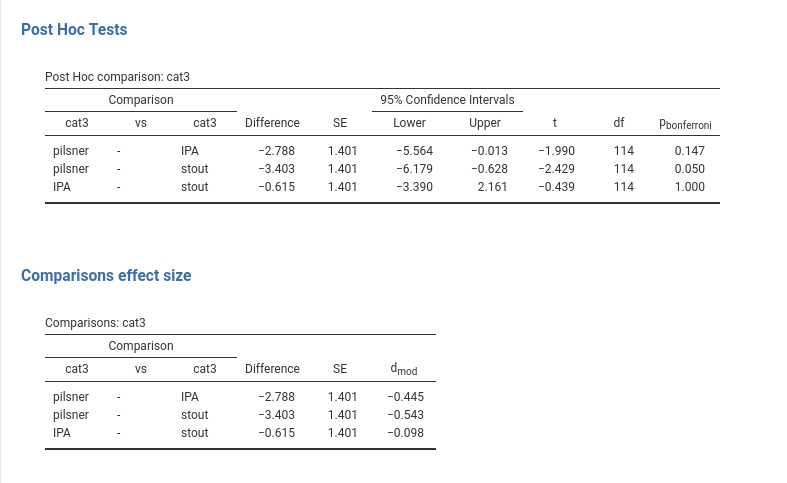
\includegraphics{bookletpics/2_anova_output6.png}

Post hoc tests are basically t-tests comparing any pair of levels of the independent variables in their dependent variable means. So, here we have the mean for the \emph{pilsner} group compared with the \emph{IPA} group, the \emph{pilsner} group compared with the \emph{stout} group, and the \emph{IPA} group compared with the \emph{stout} group. For each comparison we have the difference in means, the confidence intervals, the t-test, df, and p-value. All columns report what a simple t-test would yield, but the p-value column is different. The p-value is adjusted for multiple comparisons, meaning that the p-value is calculated to counteract the higher probability of finding something singificant when multiple tests are run. The adjustment is proportional to the number of comparisons that are tested.

Why adjusting? Well, adjustment is required when the researcher does not have an \emph{a priori} hypothesis regarding which comparison should be \emph{significant} and which should not. If one does not have a clear hypothesis, any comparison that comes out as significant will be considered as \emph{real}, so different from zero. However, when several comparisons are tested, the probability of obtaining at least one comparison as significant is not .05 (\(\alpha\)), as one expects, but higher: the more comparisons one tests, the higher the probability.

Recall that any inferential test (\emph{frequentist} tests, I should add) lays out a null-hypothesis, say \(\Delta=0\) (difference equal to zero). The t-test returns the probability of obtaining the observed result (here \(-2.788\) for \emph{pilsner} vs \emph{stout}) if we were sampling from a distribution in which \(\Delta=0\). When the p-value is low, we say that it is very unlikely that our result comes from a distribution where \(\Delta=0\), so we reject the null-hypothesis. Unlikely, however, does not mean impossible, so there is always a chance to be wrong in rejecting the null-hypothesis. If we use a significance cut-off of \(\alpha=.05\), we accept the risk of being wrong 5\% of the time, if the population difference is indeed zero. The good news is that we'll be right \(1-\alpha=.95\) (*100) of the times. However, this reasoning is valid for one test. If we run two tests, we want to take the right decision for boths, so the probability of being right in both tests is \((1-\alpha)^2=0.9025\). If we run three tests, we will be right with probability \((1-\alpha)^3=0.857375\). So, we capitalize on chance, meaning that it becomes more and more likely to get at least one test as significant, even if they all come from a population where no difference is present.

Multiple comparisons adjustment corrects the p-value in order to make a significant result more difficult to obtain. Practically, the p-value is increased proportionally to the number of comparisons that are tested. There are different methods to adjust the p-value, and they are listed in the panel as options: \emph{Bonferroni}, \emph{Tukey}, \emph{Holm}, \emph{Scheffe}, \emph{Sidak}. They are all alternative ways to adjust the p-value. The interesting dimension along which they differ is liberalism-conservativism. In statistics, a \emph{liberal} test is more likely to yield a significant result than a conservative test, \emph{ceteris paribus}. Liberal tests are more powerful but their correction of the p-value may not be enough, whereas conservative tests correct for multiplicity but may result under-powered. Bonferroni and Sidak adjustment tend to be more conservative than the others. \emph{Tukey} correction seems the more reasonable choice in most circumstances \citep{midway2020comparing}.

Recall, post hoc tests are needed when the researcher is willing to accept any significant result as worth mentioning and interpreting. On the other hand, if one has a clear pattern of means hypothesized, adjustment may not be needed and the specific comparisons may be evaluated without correction.

\hypertarget{cohens-d}{%
\section{Cohen's d}\label{cohens-d}}

Cohen's \(d\) is probably the most used effect size index to quantify a mean difference. It expresses the mean difference in a standardized scale: It is the ratio of the mean difference over the within groups standard deviation, or residual standard deviation. Unfortunately, Cohen \citep{cohen2013statistical} defined the \(d\) index for the population, and thus it is not clear how to compute it in the sample. {GAMLj} offers three options.

\begin{itemize}
\item
  Cohen's d (model SD) \(d_{mod}\): the means difference is divided by the estimated standard deviation computed based on the model residual variance.
\item
  Cohen's d (sample SD) \(d_{sample}\): the means difference is divided by the pooled standard deviation computed within each group.
\item
  Hedge's g \(g_{sample}\): the means difference is divided by the pooled standard deviation computed within each group, corrected for sample bias. The correction is the one describe by \citet{hedges2014statistical} based on the Gamma function.
\end{itemize}

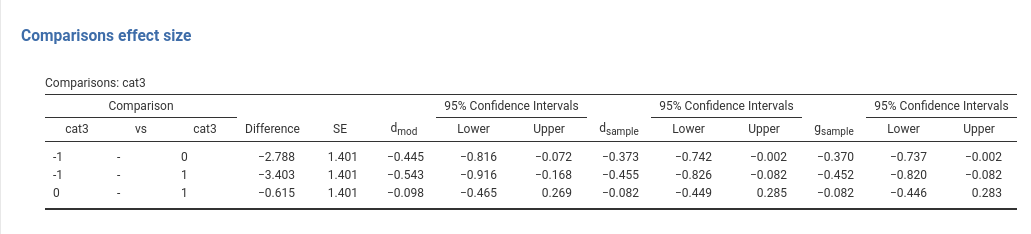
\includegraphics{bookletpics/2_anova_output8.png}

The two d's differ in their adherence with the model being estimated. The \emph{model SD} version, gives the estimated \texttt{d} after removing the variance explained by the other effects in the model, so it is the actual effect size of the comparison of the estimated marginal means. The \emph{sample SD} gives the crude standardized difference, as if the model was not estimated at all, but only the two groups were considered. The \emph{model SD} should be preferred as default index to report in a model, the \emph{sample SD} version can be useful to compare effects in the literature obtained with a different model or without a model.

Hedge's g gives a population estimate of the sample \(d\).

\hypertarget{estimated-marginal-means}{%
\section{Estimated marginal means}\label{estimated-marginal-means}}

The means that are plotted in the plot can be visualized, with their standard error and confidence intervals, by defining the variables for which we want them in the {Estimated Marginal Means}.

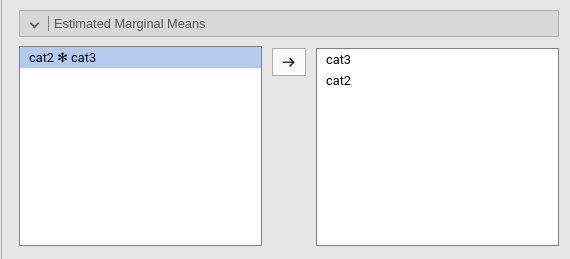
\includegraphics{bookletpics/2_anova_input7.png}
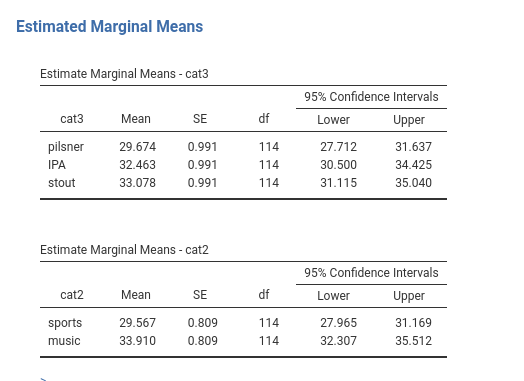
\includegraphics{bookletpics/2_anova_output7.png}

In balanced designs with only categorical {IVs {Independent Variables} }, they are the means of the groups (or combinations of groups). When there are also continuous {IVs {Independent Variables} }, they are adjusted for the continuous variables: They are the means estimated after keeping constant the continuous independent variables.

If marginal means are requested for a continuous variable, they represent the expected value of the dependent variable for three \emph{interesting} levels of the independent variable, where the \emph{interesting values} are defined as for the \emph{simple slope} technique (cf \ref{simpleslopes})

For instance, in model \ref{moderation}, if we ask for the estimated marginal means for \(x\), we obtain the following estimates:

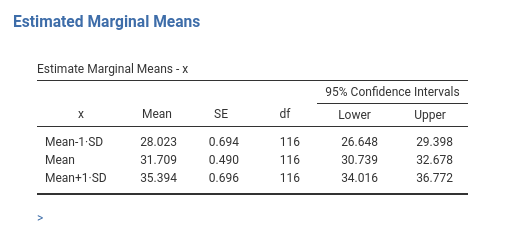
\includegraphics{bookletpics/2_moderation_output1.png}

meaning that, based on the model, we expect the number of smiles (\texttt{ycont}) to be 28.03 for low level of beers (1 SD below average of \texttt{x}), 31.7 for the average level of beers (average of \texttt{x}), and 35.9 for high levels of beers (1 SD above average of \texttt{x}).

\hypertarget{ancova}{%
\section{Categorical and Continuous IVs}\label{ancova}}

\begin{flushright} AKA: ANCOVA  \end{flushright}

We now insert in the model also \(x\), so we have both categorical and continuous {IVs {Independent Variables} }. This model was once called \emph{ANCOVA}, but it did not allow for interactions. We simply call it a GLM.

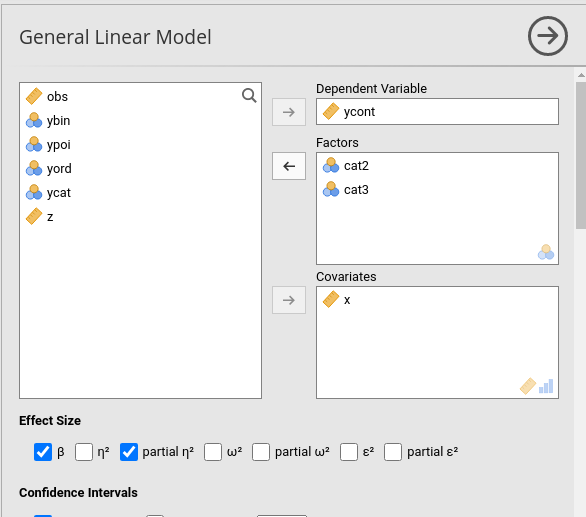
\includegraphics{bookletpics/2_ancova_input1.png}

Keeping up with an old (SPSS?) tradition, {GAMLj} does not automatically insert into the model interactions involving a continuous variable, so if one needs them, they should be added manually (see below). For the moment, here is our model.

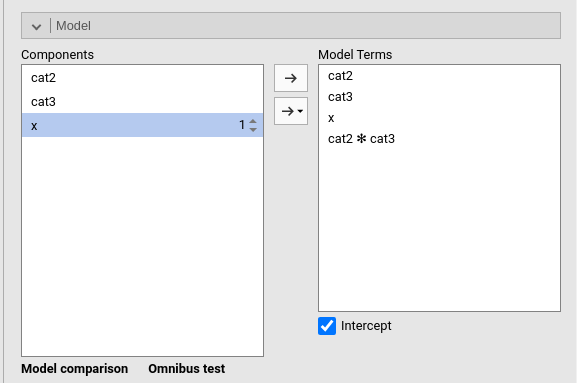
\includegraphics{bookletpics/2_ancova_input2.png}

\hypertarget{results-tables}{%
\subsection{Results tables}\label{results-tables}}

\includegraphics{bookletpics/2_ancova_output1.png}

Combining categorical and continuous {IVs {Independent Variables} } does not really change the way we interpret the results. We interpret the continuous variable effect like we did for the continuous variables GLM (\ref{multiregression}) and the categorical independent variables effects as we did for the GLM with categorical variables (\ref{anova}). So, in the {Model Fit} Table we found the variance explained by all the effects combined, in the {ANOVA Omnibus Tests} Table we find the explained variances and their tests, and in the {Parameter Estimates (Coefficients)} Table we find the coefficients. We just need to keep in mind that all the effects are computed keeping constant the other variables, so we can use this kind of model to \emph{covariate} variables that may have spurious effects. That is why in the last century this model was called \emph{ANalysis of COVAriance}. At that time, one assumption of this analysis was that there was no interaction between the categorical variables and the continuous variables. Nowadays, we can release the assumption, and just test the interaction, in case is there.

\hypertarget{moderation2}{%
\section{Categorical and Continuous Interactions}\label{moderation2}}

There is nothing special about interactions between continuous and categorical variables, they just test a moderation model. To obtain the interactions we select all variables in the {Model} panel and click the arrow to bring them in the \texttt{Model\ Terms} field.

\includegraphics{bookletpics/2_ancova_input3.png}

Upon updating the model, the results update as well, and now we can check the main effects, the 2-way interactions and the 3-way interaction. We focus on the variances explained and F-tests.

\includegraphics{bookletpics/2_ancova_output3.png}

When the model features interactions of different orders, it is a good idea to start the interpretation from the highest order interaction, in our case the 3-way interaction. Here it seems to be different from zero, F(2,108)=6.340, p=.002, \(p\eta^2=.105\).
This means that the 2-way interaction \texttt{x\ *\ cat3} is different at different levels of \texttt{cat2}. In general, a 3-way interaction can be interpreted by picking a moderator (any will do, the interaction is symmetrical), and saying that the other two variables interaction changes at different levels of the moderator.

Upon finding a higher order interaction, one wants to plot it and interpret its direction. This is because the higher order interaction shows a pattern of results that is more specific then lower order effects. In fact, lower order effects are always interpreted \emph{on average}, so they are less specific than the higher order effect. Practically, the \texttt{cat2\ *\ cat3} significant interaction in our results is not very informative given these results, because it says that \emph{on average}, meaning averaging across levels of \texttt{x}, there is an interaction between type of bar and type of beer. But we know from the significant 3-way interaction that the 2-way interaction changes at different levels of \texttt{x}, so it is not really important its value on average.

If the 3-way interaction was not significant, or minuscule for our standards, we would simply start probing the lower order effects.

\hypertarget{plot}{%
\subsection{Plot}\label{plot}}

To visualize the 3-way interaction, we should pick the two variables that create the 2-way interaction we want to explore, and a moderator: the 2-way interaction is displayed for different levels of the moderator. Here we want to see the effect of beers (\texttt{x}) by type of beers (\texttt{cat3}), displayed at different levels of type of bar \texttt{cat2}.

\includegraphics{bookletpics/2_ancova_input4.png}
\includegraphics{bookletpics/2_ancova_output4a.png}
\includegraphics{bookletpics/2_ancova_output4b.png}

The interpretation can follow these lines: In \emph{sports bar}, the effect of beers on smiles is generally positive, it is stronger for \emph{stout} and IPA beers, and weaker for \emph{pilsner}. In \emph{music bar}, the effect of beers on smiles is positive as well, but stronger for \emph{stout} and weaker and very similar for \emph{pilsner} and \emph{IPA}. The fact that the two patterns can be described differently across types of bar is justified by the significant 3-way interaction.

\hypertarget{simple-effects}{%
\subsection{Simple Effects}\label{simple-effects}}

We can quantify and tests all the effects depicted in the plots by asking for \emph{simple effects} analysis. We just need to pick the variable for which we want to study the effects, and select the moderators: the focal variable effect will be estimated and tested for each combination of the moderators values.

\includegraphics{bookletpics/2_ancova_input5.png}
\includegraphics{bookletpics/2_ancova_output5.png}

The interpretation of these effects follows what we have done for the 2-way interaction before (\ref{simpleslopes}). However, because we have a 3-way interaction, we can also probe for \emph{simple interactions}.

\hypertarget{simpleinteractions}{%
\section{Simple Interactions}\label{simpleinteractions}}

\emph{Simple interactions} are simple effects, in which the focal effect is an interaction. We can ask for this analysis by selecting {Simple Interaction} option.

\includegraphics{bookletpics/2_ancova_input6.png}
\includegraphics{bookletpics/2_ancova_output6.png}

This analysis is useful to probe high order interaction. Here we see the \texttt{x\ *\ cat3} interaction computed at the two levels of \texttt{cat2}. So, we can say that for the group \emph{music}, the interaction is present, whereas for group \emph{sports}, the \texttt{x\ *\ cat3} interaction is not statistically significant.

\hypertarget{model-comparison-approach}{%
\section{Model-comparison approach}\label{model-comparison-approach}}

\hypertarget{the-method}{%
\subsection{The Method}\label{the-method}}

We have touched upon the fact that many tests and indices in the linear model can be derived by the comparison between two models, one being our full model, the other being a nested model \citep{judd2017data}, (cf.~Appendix \ref{appendixa}). A nested model is simply a model that, compared with the full model, lacks some terms, and does not have any term not present in the full model. {GAMLj} allows custom model comparisons by flagging the option {Activate} under {Model Comparison}.

\includegraphics{bookletpics/2_modelcomparison_input1.png}

Comparing models is useful when we want to estimate the variance explained by a set of effects \citep{cohen2014applied}, and test this variance. For instance, one may have an experiment with a series of possible confounding variables, and the aim is to estimate the variance explained by the experimental factors (all together) over and beyond the confounding variables explained variances. Another case may be a model in which socio-economical variables (e.g income, real-estate properties, etc) and psychological variables (e.g self-esteem, emotional regulations) are compared in their ability to explain an outcome (say \emph{happyness}). Besides each individual variable effect size, the researcher may be interested in estimating the variance explained by \emph{economics} vs the variance explained by \emph{psychology}. A model-comparison approach may be helpful.

In our running example, we would like to estimate and test the impact of \emph{beer} (\(x\)) and \emph{extraversion} (\(z\)) over and beyond the effect of \emph{type of bar} (\(cat2\)) and \emph{type of beer} (\(cat3\)). Our full model involves all mentioned variables, plus the interaction between the factors (see Figure above). We now need to specify a smaller model, which includes only the categorical variables and their interaction. We set this model in the {Nested Model} field.

\includegraphics{bookletpics/2_modelcomparison_input2.png}

What we are saying to the module is to estimate a full model, then estimate a model with only the categorical variables, and compare the fit (\(R^2\)). The difference between the two \(R^2\)'s is the variance uniquely explained by the terms present only in the full model, in our case \(x\) and \(z\). The output is the following:

\includegraphics{bookletpics/2_modelcomparison_output2.png}

Thus, the full model explains \(R^2=.406\) (*100) of the variance of the dependent variable, the Nested model, without \(x\) and \(z\) explains \(R^2=.162\) (*100) of the variance. Their difference, \(\Delta R^2=.245\) is the variance uniquely due to \(x\) and \(z\) together.

\hypertarget{types-of-tests}{%
\subsection{Types of tests}\label{types-of-tests}}

In the General Linear Model, all tests are usually performed with F-test. The F-test works fine and has a solid tradition in statistics. Therefore, it is perfectly fine to use it also to compare models. After all, model-comparison entails comparing variances explained, which is the F-test job since more than 100 years. Recently, the statistical literature has made another test popular in model-comparison methods: The LRT, log-likelihood ratio test. This test is very useful for models estimated maximizing the log-likelihood of the data given the model, such as the generalized linear model or (with some caveats), the mixed model. For those passionate about the LRT, {GAMLj} offers the option to obtain the LRT also for the GLM, by selecting {LRT} under {Omnibus test}. In the GLM, the p-values based on the F-test and the LRT are usually very similar.

\includegraphics{bookletpics/2_modelcomparison_input3.png}
\includegraphics{bookletpics/2_modelcomparison_output3.png}

\hypertarget{not-necessary-model-comparisons}{%
\subsection{Not necessary model-comparisons}\label{not-necessary-model-comparisons}}

One should not be carried away by model-comparisons (the custom version of the method), because it is seldom useful and the \emph{usual} estimates and tests of the linear model are already some sort of model-comparisons. Recall, for instance, the model with \(x\) and \(z\) as independent variables.

\includegraphics{bookletpics/2_modelcomparison_input4.png}
\includegraphics{bookletpics/2_modelcomparison_output4.png}

Notice that we selected \(\eta^2\) as an additional effect size index. First, if we make a model-comparison with an intercept only model, we get exactly the \(R^2\) we obtained in the standard analysis. This is because the \emph{usual} \(R^2\) is already a fit comparison between our full model and an intercept-only model (cf appendix \ref{appendixa}).

\includegraphics{bookletpics/2_modelcomparison_input5.png}
\includegraphics{bookletpics/2_modelcomparison_output5.png}

Second, if we now add to the nested model the variable \(z\), we are comparing a model with \(x\) and \(z\) as terms with a model with only \(z\), so we are estimating the contribution of \(x\) to the explained variance.
\includegraphics{bookletpics/2_modelcomparison_input6.png}
\includegraphics{bookletpics/2_modelcomparison_output6.png}

The \(\Delta R^2\) is now .317, with \texttt{F(1,117)=56.68}, which is exactly the \(\eta^2\) of the \(x\) in the full model, with the same F, df, and p-value. The effect of \(x\) is already a result of a model-comparison test, so we do not need to test it explicitly.

\hypertarget{hierarchical-regression}{%
\subsection{Hierarchical regression}\label{hierarchical-regression}}

The model-comparison approach allows estimating what many people call \emph{hierarchical regression}. Hierarchical regression is an analytic strategy, it is not a statistical model. By \emph{hierarchical regression} one means the estimation of the coefficients of different {IV {Independent Variable} } in different models, containing different sets of {IV {Independent Variable} }. For instance, one may want to estimate the effects of \(cat2\) and \(cat3\) independently of \(x\) and \(z\), but the effects of \(x\) and \(z\) keeping constant \(cat2\) and \(cat3\). In a hierachical regression software, one specify a first block with \(cat2\) and \(cat3\), and a second block with all variables. The software would estimate two models, and produce a recap table with the coefficients obtained in the first model for \(cat2\) and \(cat3\), and the results obtained in the second model for \(x\) and \(z\). Possibly, the \(\Delta R^2\) is also produced.

This analytic strategy is rarely useful, but if this is really the intent of the analyst, one can use {GAMLj} to estimate two different models to obtain the coefficients, and then obtain the \(\Delta R^2\) with a model-comparison approach. Alternatively, one can use {jamovi} \texttt{regression} command, which allows to specify blocks. Results will be identical, only the tables will be organized in different ways.

\hypertarget{assumptions-checks}{%
\section{Assumptions checks}\label{assumptions-checks}}

The GLM is based on several assumptions, a few of which are popular and they are regularly tested or at least checked. We should start saying that assumptions are idealized scenarios in which data show a required property. They are needed to unsure that the expected results (F-test, p-values, etc.) posses the expected properties (unbiasedness, consistency, etc). In other words, the assumptions are required so we can trust the results, cf. \citet{nimon} and \citet{glass1972consequences} for details.

Being idealized scenarios, the observed data are never perfectly abiding by the assumptions, but they approximate the required property with different degrees. The better a property is approximated, the more we can trust the results. The worse is approximated, the more doubts we should cast on our results. Because the properties required by the assumptions are only approximated to a certain degree, assumptions cannot be evaluated only using an inferential test. Inferential tests tend to be interpret as ``significant'' vs ``not significant'', and such a dichotomy is not always useful when evaluating assumptions. For this reason, {GAMLj} provides both inferential tests and graphical methods to assess the appropriateness of the data with respect of the assumptions.

Here we focus on the homoschedasticity and normality of residuals assumptions.

\hypertarget{homosched}{%
\subsection{Homoschedasticity}\label{homosched}}

By \emph{Homoschedasticity} we mean that the variance of the residuals is constant around the predicted values, that this the residuals spread around the predicted values at more or less the same distance along the model predictions. In other words, the spread of the clouds of points representing the {DV {Dependent Variable} } as a function of the {IV {Independent Variable} } is constant. When the spread is not constant, we have \emph{Heteroschedasticity}. Here are two exemplifications:

\includegraphics{bookletpics/2_assumptions_theory1.png}

In cases where the independent variables are categorical, the assumption requires that the variances within groups are more or less the same across groups.

The idea is that the error term, which is the residuals variance, should be representative of the residual variance across all values of the predicted values. This is \emph{Homoschedasticity}. On the contrary, the error term is not representative of the whole model if the variance of the resifuals is different for different predicted values, because it would be larger or smaller in different parts of the model. That is \emph{Heteroschedasticity}. \emph{Homoschedasticity} ensures that the standard errors associated with the estimates are correct, and thus are the inferential tests and the p-values one obtains along the coefficients estimates.

To evaluate the \emph{Homoschedasticity} we can use two inferential tests and one graphical method.

\includegraphics{bookletpics/2_assumptions_input1.png}

The tests are the Breusch-Pagan test and the Levene's test.

\includegraphics{bookletpics/2_assumptions_output1.png}

Both tests test the null-hypothesis that the variance of the residuals do not change along the predicted values, so the assumption is met when they are not significant. A significant test, on the contrary, indicates that the residuals variance departs from the assumption of homogeneity, and thus we should cast some doubt on the validity of the results.

The Breusch-Pagan is defined for any GLM, so it is estimated whatever our {IVs {Independent Variables} } are. The Levene's test is defined only for categorical {IVs {Independent Variables} }, so it is not produced when the {IVs {Independent Variables} } are all continuous.

Graphically, we can check the {Residuals-Predicted plot}. This plot depicts the residuals (in the Y-axis) as a function of the predicted (on the X-axis), so it makes it easy to see whether the spread of the cloud of points changes along the X-axis. The assumption is approximated well when the depicted cloud of points has more or less the same spread along the whole plot. Examples may be:

\includegraphics{bookletpics/2_assumptions_output2.png}

\hypertarget{normality-of-residuals}{%
\subsection{Normality of residuals}\label{normality-of-residuals}}

To guarantee unbiased inferential tests, that is valid p-values, residuals should be normally distributed (Gaussian). {GAMLj} provides the Kolmogorov-Smirnov test, the Shapiro-Wilk test, the histogram plot and the Q-Q plot to assess this assumption.

\includegraphics{bookletpics/2_assumptions_input3.png}

\includegraphics{bookletpics/2_assumptions_output3.png}

Both inferential tests share the null-hypothesis that the distribution is normal (Gaussian), thus a non-significant test indicates lack of evidence against the assumption, whereas a significant test indicates departure from the assumptions. Shapiro-Wilk seems more powerful, so it should be preferred in small samples, whereas the Kolmogorov-Smirnov may be more appropriate in large samples.

The first graphical method is a simple histogram of the residuals, on which the module overlays a perfectly normal curve with the same mean and standard deviation of the observed one, so the comparison becomes easier.

\includegraphics{bookletpics/2_assumptions_output4.png}

Here we want to check that our distribution is not too far away from a normal distribution, especially with regards of the main properties of the normal one: symmetry and increasing density (frequency of cases) closer to the mean.

Another popular graphical method is the Q-Q plot.

\includegraphics{bookletpics/2_assumptions_output5.png}

The Q-Q plot plots the theoretical quantiles (percentiles) of a perfectly normally distributed variable with the quantiles of our observed distribution. The closer our distribution to the normal one, the closer the scattered points will be to the 45 degrees line.

\hypertarget{violations-remedies}{%
\section{Violations Remedies}\label{violations-remedies}}

\includegraphics{bookletpics/2_options_input1.png}

\hypertarget{robust-standard-error}{%
\subsection{Robust Standard Error}\label{robust-standard-error}}

Whereas it is often the case that both assumptions are violated, the violation of \emph{homoschedasticity} and the violation of \emph{normality of the residuals} have different remedies.

Lack of \emph{homoschedasticity}, that is \emph{heteroschedasticity}, can be counteracted by using a robust method to compute the standard errors. Whereas \emph{robust} estimations is a very general term, in the context of the GLM it usually means \emph{robust against heteroschedasticity}. {GAMLj} offers \emph{robust} standard error in the {Options} panel, under {SE method}. When \texttt{Robust} is selected, one can choose the algorithm to compute the HC (\textbf{H}eteschadasticity-\textbf{C}onsistent) standard errors. {GAMLj} implements these algorithms as implemented in the sandwich R package, setting \texttt{HC3} as default as recommended by the package authors.

Setting the SE method to robust updates all results related with inferential tests, and thus the results will be different, and more accurate, proportionally to the strength of the assumption violation.

\hypertarget{bootstrap-confidence-intervals}{%
\subsection{Bootstrap Confidence Intervals}\label{bootstrap-confidence-intervals}}

When the residuals are not normally distributed, or when other assumptions are suspicious,
one can rely on Bootstrap Confidence Intervals. The advantage of the bootstrap C.I. is that they do not assume any shape for the residual distribution, because their boundaries are estimated by resampling the observed distribution (cf.~Bootstrapping, and \citet{efron1994introduction}).

{GAMLj} offers two methods to compute bootstrap confidence intervals. The \texttt{percent} and the \texttt{BCa} method. The \texttt{percent} method entails building a bootstrap distribution of estimates and select the \(100 \cdot (\alpha/2)\)th and the \(100 \cdot (1-{\alpha /2})\)th percentile of the distribution as the boundary of the interval. In other words, for the 95\% C.I (where \(\alpha=.05\)), it selects the 2.5th and 97.5th percentile of the bootstrap distribution. The \texttt{BCa} method stands for \emph{Bias corrected and accelerated} method. The method corrects the percentile values depending on the skewness of the bootstrap estimates distribution and the offset of the distribution mean compared with the observed estimate. The specialized literature seems to indicate that for generic situations, the \emph{percent} method gives more accurate results (cf., for instance, \citet{jung2019comparison}).

The number of bootstrap resampling is set to 1000, but for reliable and replicable results one can set it to 5000 or 10000. Just keep in mind that resampling means to estimate a full model for every bootstrap sample, so the process might be quite time-consuming for large models.

\hypertarget{gzlm}{%
\chapter{The Generalized Linear Model}\label{gzlm}}

{ Draft version, mistakes may be around }

\hypertarget{gzlmintro}{%
\section{Introduction}\label{gzlmintro}}

In the general linear model (cf.~\ref{glm}) the dependent variable must be a quantitative variable: It should express quantities, such that its values can retain all properties of the numbers: 1 is less than 2, 4 is 2*2. In this way, the mean, the variances and all the estimates can make sense. We have also seen that the GLM assumes the residuals being normally distributed, which is akin to saying that the dependent variable is normally distribute (a part from the {IVs {Independent Variables} } influence). There are many research designs that require the dependent variable to be not-normally distributed or not even quantitative. One may want to predict the vote in a referendum, the number of smartphone owned by individuals, the sex of the offspring of a herd, a choice between two or more product colors in a marketing study. In all these circumstances, the GLM cannot be applied.

We still want to use a linear model, though, because we know very well how to estimate it and interpret it. So, instead of forgoing the linear model, we change the way the linear model predicts the dependent variable, such that the estimates are unbiased and reasonable even when the dependent variable values are not quantities, or they are clearly not normally distributed.

Here comes the \emph{generalized linear model}. Consider the standard regression model.

\[
\hat{y_i}=a+b x_i
\]
The \(\hat{y_i}\) are the predicted values, meaning the points lying on the regression line, that correspond to the expected (average) values of \(y\) for any possible value of \(x\). In the GLM, the predicted values have the same scale of the observed values: This is because \(\hat{y_i}\) can take any value (the straight line is defined for any possible value in the Y-axis), and so can \(y_i\), the observed values. When the variable is not quantitative, or it has a weird distribution, we cannot be sure that the predicted values will make sense. If one is predicting a probability, for instance, the observed values vary from 0 to 1, and thus the predicted values of a GLM will surely be nonsense, because the line will overcome the 0-1 boundaries and predicts probabilities of, say, 10 or -30, that are not admissible. If the predicted values make no sense, the model make no sense.

If we, however, express the predicted values as a transformation of the dependent variable, we can choose the right transformation to be sure that the predicted values will make sense. The transformation is called the \emph{link function} (\(f()\)), and one can pick different link functions to accommodate different types of dependent variables. The \emph{generalized linear model} is a linear model in which the predicted values are expressed as a transformation of the dependent variable:

\[
f(\hat{y_i})=a+b x_i
\]
In addition to predicting a transformation of the dependent variable, the generalized linear model does not assume the dependent variable to be normally distributed, but allows assuming different families of distribution: Binomial, multinomial, Poisson, etc.

Combining a particular link function with a distribution makes a particular application of the generalized linear model. The combination of link function and distribution makes a particular application a model suitable for predicting a particular type of dependent variable. Here is a brief recap of the generalized linear models that can be estimated with {GAMLj}.

Model

Link Function

Distribution

DV type

Logistic Model

Logit

Binomial

Dichotomous

Probit Model

Inverse cumulative normal

Binomial

Dichotomous

Multinomial Model

Logit

Multinomial

Categorical

Ordinal Model

Cumulative Logit

Logit

Ordinal

Poisson Model

Log

Poisson

Count (frequencies)

Negative Binomial Model

Log

Negative binomial

Count (frequencies)

We are going to explore all these models, highlighting their specificity but keeping in mind that all techiques and methods doable to the GLM (cf.~\ref{glm}) can be applied also to the models within the generalized linear model.

As a general reference for the material discussed in this chapter, the book \citet{agresticategorical} is a great source of information and a precise guide to the statistical details.

\hypertarget{logistic}{%
\section{Logistic Model}\label{logistic}}

\hypertarget{the-rationale}{%
\subsection{The rationale}\label{the-rationale}}

A logistic model can be estimated when the dependent variable features two groups, or two levels. The necessity to change the GLM into a different linear model becomes clear by inspecting a scatterplot between a continuous independent variable and a dichotomous dependent variable.

\includegraphics{bookletpics/3_logistic_plot1.png}

It is clear that the dependent variable scores can only be 0 or 1, and that the scatterplot will always present two horizontal stripes points, forming a cloud that cannot be represented well by a straight line. A straight line that will feature predicted values surely above 1 and below 0, providing nonsensical predicted values. The residuals, furthermore, will depend on the predicted values (cf heteroschedasticity in \ref{homosched}), because the line will cross a strip once (so residual is zero) and depart from it everafter (increasing the residual variance).

The solution is to change the form of predicted values such that any values can be a sensible predicted value. To achieve this, we should first notice that when one has a dichotomous dependent variable, what one is predicting is the probability of being in the group scoring 1. Indeed, the predicted values are the expected (average) values of \(y\) for each given \(x_i\). The average value of a dichotomous variable is
\[
E(y)={n_1 \over N}
\]
where \(n_1\) is the number of cases in group 1, and N is the total sample. \(E(y)\), however, is the probability of being in group 1. Thus, \(p(x=1)=E(y)\), which we simply call \(p\).

So, the aim of the logistic model is to estimate how the probability of being in group 1 rather than 0 depends on the {IVs {Independent Variables} } scores. The probability scale, varying from 0 to 1, is not suitable to be fit by a straight line. We can change this by predicting the \emph{odd} of the probability, namely:

\[
odd={p \over {1-p}}
\]

The odd frees us from the upper boundary of 1, because any positive value expressed in odd can be sensible predicted value. For each positive value, one can always transform it back and get back a probability. The problems are negative values, that a straight line will always yield. Since the odd cannot be negative, we need to apply to it another transformation, namely the logarithm transformation. A logarithmic transformation transforms a positively-valued variable into a variable with all possible values, positive and negative. The function that expresses a probability into a variable admitting all possible values is the logit function:

\[
logit(y)={log \left( {p \over 1-p} \right)}
\]

The logistic model is a linear model predicted the logit

\[
logit(\hat{y})=a+b_1  x_1+b_2 x_2+ ...
\]

Everything we can do with a linear model can be done with the logistic model, we just need to keep in mind that the interpretation of the results must consider the fact that the predicted values have a logistic scale, and not the original dependent variable scale.

\hypertarget{logisticestim}{%
\subsection{Model Estimation}\label{logisticestim}}

We can use our \emph{manymodels} dataset to see an example of a logistic model. The dataset contains a dichotomous dependent variables called \texttt{ybin}, which features two groups. To keep up with our cover story, we can imaging it to represent visiting the toilet behavior. \(ybin=1\) means that the customer has visited the bar restroom, \(ybin=0\) means that the client has not visited the restroom that evening.

\includegraphics{bookletpics/3_logistic_freq1.png}

The aim of the model is to estimate the relationship between number of beers (\(x\)) and the probability of visiting the restroom (\(ybin\)).

In {GAMLj} we launch \texttt{Generalized\ Linear\ Models} menu of the \texttt{Linear\ Models} icon. The first part of the user interface allows selecting the appropriated model. In our case, we selected {Logistic} because our dependent variable is a dichotomous variable.

\includegraphics[width=0.9\linewidth]{bookletpics/3_logistic_input1}

Once we have selected the model, we can set up the variables in the variables role fields, as we did in the GLM (cf.~\ref{glminput}).

\includegraphics{bookletpics/3_logistic_input2.png}

\hypertarget{logisticrecap}{%
\subsection{Model Recap}\label{logisticrecap}}

\includegraphics[width=0.9\linewidth]{bookletpics/3_logistic_output1}

In the {Model Info} table we find a set of properties of the estimated model. The most important one to check is described in the \texttt{direction} row. When the dependent variable is dichotomous, in fact, the direction of the probability is arbitrary, so we need to know which group is predicted. {GAMLj} models the probability of being in the group with the ``largest'' label value, after ordering the value labels. In our case, it models the probability of being in group \texttt{ybin=1} over the probability of being in group \texttt{ybin=0}. This is indicated in the \texttt{direction} row of the table.

\hypertarget{model-fit}{%
\subsection{Model Fit}\label{model-fit}}

\includegraphics{bookletpics/3_logistic_output2.png}

First, the model R-squared is produced with its inferential test, in this case a Chi-square test. This provides a test of the ability of the model to predict the dependent variable better than chances. The R-squared is the McFadden's pseudo R squared (cf GAMLj help
). We can interpret it as the proportion of reduction of error, or the proportion of increased accuracy in predicting the dependent variable using our model as compared with a model without independent variables (cf.~Appendix \ref{appendixa}). The adjusted \(R^2\) is the population \(R^2\) estimate.

The additional indices reported in {Additional indices} reports other indices useful for model comparisons or evaluation of models, especially for other types of generalized linear models. They are rather technical, and we'll not discuss them here.

\hypertarget{omnibus-tests-1}{%
\subsection{Omnibus Tests}\label{omnibus-tests-1}}

As for the GLM, we have omnibus tests for the effects of our {IVs {Independent Variables} }. They are expecially useful when dealing with categorical independent variables, because with continuous independent variables they are redundant as compare with the coefficients tests. With one {IV {Independent Variable} }, the omnibus test is equivalent to the model fit test.

\includegraphics{bookletpics/3_logistic_output3.png}

\hypertarget{coefficients-1}{%
\subsection{Coefficients}\label{coefficients-1}}

\includegraphics{bookletpics/3_logistic_output4.png}

With continuous {IVs {Independent Variables} }, the coefficients \texttt{Estimates} are the most interesting parameters.
The \texttt{Estimate} column reports the regression coefficients. Their interpretation should be based on the fact that the predicted values scale is the logit scale. Thus, as regard the effect of \(x\), we can say that for one unit more in \(x\), the logit of the probability of being in the group \(ybin=1\) increases of one 1.53 units. In our cover story, for one more beer the logit of visiting the restroom increases of one unit. Being positive, we can conclude that the more you drink, the higher the probability of visiting the restroom. Being statistically significant (z-test=4.73, p.\textless.001), we can conclude tha the effect is different from zero.

\hypertarget{odd-ratios-expb}{%
\subsection{Odd ratios exp(B)}\label{odd-ratios-expb}}

The issue here is that it is very difficult to fathom the practical size of the effect. Is\\
1.53 units increase in the logit scale a big or small increase? Honestly, nobody knows, because the logarithm scale is difficult to master, and even if one could, the readers of the results would probably not. So, we interpret the \texttt{exp(B)} parameter, which is the logit after removing the logarithm scale. The logarithm scale is removed by simply passing the logit to the exponential function, hence the notation \texttt{exp(B)}. If we remove the logarithm scale, we are left with the odd scale. However, we should pay attention to what happens to the coefficients when the scale is changed from the logit to the odd. Two pieces of information are important here. First, recall that the \(b\) coefficient in a linear model (any linear model) is the difference in the predicted values for two consecutive values of the independent variable. That is

\[
b=\hat{y}_{(x=1)}-\hat{y}_{(x=0)}
\]
In the logistic model, we have
\[
b=log(odd_{(x=1)})-log(odd_{(x=0)})
\]
The second piece of information is that when you take the exponential function of a difference between two logarithms, the result is the ratio between the logarithms arguments. That is

\[
exp(log(a)-log(b))={a \over b}
\]
Thus, if we take the exponential function of the logit B, we obtain the ratio between two odds

\[
exp(b)={odd_{(x=1)} \over odd_{(x=0)}}
\]

Therefore, \texttt{exp(B)} is a ratio between two odds, computed at two consecutive values of the independent variable. That is why it is called the \emph{odd ratio}. It is \emph{the rate of change of the odd as you increase the independent variable of one unit}. In other words, it indicates how many times the odd changes as one increases the exponential function of one unit. In our example \texttt{exp(B)=4.62}, so, for every beer more, the odd of going to the restroom increases of 4.62 times.

The odd ratio is the standard effect size used in logistic regression, but it is not the only one. In different disciplines other ways to quantify the logistic effects are used. {GAMLj} provides the most common ones: \emph{Marginal effects} and \emph{Relative Risk}. Now we discuss the former because it is more appropriate with continuous {IVs {Independent Variables} }. We discuss the RR when we deal with categorical {IV {Independent Variable} } (cf \ref{gzlmanova})

\includegraphics{bookletpics/3_logistic_input3.png}

\hypertarget{logisticcontmarginal}{%
\subsection{Marginal effects}\label{logisticcontmarginal}}

In the same way that the \texttt{exp(B)} gets rid of the log scale, marginal effects get rid of the odd scale \citep{agresti2018simple}. If we get rid of the odd scale, we are back in the probability scale. Let's see our model in probability scale, by asking the plot of the predicted values in the {Plots} panel (as we did in GLM \ref{glmplot}).

\includegraphics{bookletpics/3_logistic_plot2.png}

First, notice that our model is not linear, because the logistic model is linear for the logit outcome. The plots represents the predicted values in probabilities, so the linearity is lost, but the predicted values make sense. Second, recall that the coefficient of a regression tells us in which direction and how steep is the change in the predicted values as one increases the independent variables. The problem with probability-scaled predicted values is that the direction and size of the change is not constant along the independent variable scores.

\includegraphics{bookletpics/3_logistic_plot3.png}

In the model above, for instance, for \(x=-2\) we can see a mildly positive increase, whereas for \(x=0\) the increase is very steep, which becomes almost flat for \(x=2\). Each of this possible increases (or change in probability) is a marginal effect. However, if we want to quantify the increase (or change) in probability due to the increase in the {IV {Independent Variable} }, we have a different marginal effect for each value of \(x\). But we can compute them all (for all observed values of \(x\)) and take the average: This is the average marginal effects (AME) produced by {GAMLj}.

\includegraphics{bookletpics/3_logistic_output5.png}

Thus, we can say that on average, the probability of visiting the restroom (\(ybin=1\)) increases of .271 as you increase beer (\(x\)) of one unit.
Please consult \citet{thomas} for more details and technical information.

\hypertarget{multiple-ivs}{%
\subsection{Multiple IVs}\label{multiple-ivs}}

Adding independent variables in the logistic regression, as well as interaction terms, follows the same principles used for the GLM (\ref{glm}). The coefficients are interpreted as partial coefficients, keeping constant the other independent variables. If interactions are included, the linear effects are interpreted as \emph{main effects} (averaged across leves of the moderator). Simple effects analysis and simple slopes plots can be obtained as we did in the GLM applications.

\hypertarget{gzlmanova}{%
\section{Logistic with Catecorical IVs}\label{gzlmanova}}

We know that the GLM can accommodate categorical {IVs {Independent Variables} }, and so does the logistic model. Categorical {IVs {Independent Variables} } are cast into the model using contrast variables (cf.~\ref{dummies}), their coefficients represent group comparisons, and their omnibus tests inform us on the effect of the categorical variable on the probability of being in the group \(y=1\) rather than the group \(y=0\).

We are going to exemplify this model using the \texttt{manymodels} dataset, using \texttt{cat2} and \texttt{cat3} as our categorical {IVs {Independent Variables} }. Recall we use as a cover story the type of beer drunk for \texttt{cat3} and the type of bar for \texttt{cat2}.

\includegraphics{bookletpics/3_logistic_output6.png}

\hypertarget{model-estimation}{%
\subsection{Model Estimation}\label{model-estimation}}

Now we want to establish possible differences among these groups in the probability of visiting the restroom (\(ybin=1\)). We set up a logistic model in which \texttt{cat2} and \texttt{cat3} are factors, meaning categorical {IVs {Independent Variables} }.

\includegraphics{bookletpics/3_logistic_input4.png}

As usual in {GAMLj}, in the presence of categorical {IVs {Independent Variables} } the model is automatically set up with main effects and interactions.

\includegraphics{bookletpics/3_logistic_input5.png}

\hypertarget{model-fit-1}{%
\subsection{Model Fit}\label{model-fit-1}}

\includegraphics{bookletpics/3_logistic_output7.png}

The output tables concerning the fit of the model do not really change when the independent variables are categorical. The \(R^2\) indicates the advantage of fit of our model as compared with a intercept-only model, the \(R^2_{adj}\) estimate the quantity in the population, and the inferential test (\(\chi^2\)) indicates whether our model predicts the dependent variable better than chances. More precisely, the model fit indicates if and how much our model predicts the probability of group membership better than just saying that the probability of being in group 1 is equal for every case and it is the number of cases in group 1 divided by the total number of cases.

\hypertarget{omnibus-tests-2}{%
\subsection{Omnibus Tests}\label{omnibus-tests-2}}

With categorical {IVs {Independent Variables} }, the crucial table is the {Omnibus Tests} table. Here we find the inferential tests for the main effects and the interactions.

\includegraphics{bookletpics/3_logistic_output8.png}

We can see that we obtain a non significant main effect for \texttt{cat3} indicating that there is not enough evidence to show that the three groups defined by \texttt{cat3} have different probabilities to go to the restroom (\(y=1\)). The lack of interaction indicates that the effect of \texttt{cat3} is not different across levels of \texttt{cat2}. We do find a main effects of \texttt{cat2}, with \(\chi^2(1)=15.73\), p.\textless.001. This means that the probability of being in \(ybin=1\) group is different in the two groups defined by \texttt{cat2}. People in the two types of bar visit the restroom with different probability. To interpret the direction of the effect, we can look at the plot

\hypertarget{plots-1}{%
\subsection{Plots}\label{plots-1}}

The plot depicts the average probability of \(ybin=1\) for the groups defined by the variables we ask the plot for. In our case, we ask the plot for \texttt{cat2}.

\includegraphics{bookletpics/3_logistic_input6.png}

\includegraphics{bookletpics/3_logistic_plot4.png}

We can see that the group \texttt{music} has a higher probability of visiting the restroom than the group \texttt{sport}. We can see the same information in the \emph{Estimated Marginal Means}

\hypertarget{estimated-marginal-means-1}{%
\subsection{Estimated Marginal Means}\label{estimated-marginal-means-1}}

Estimated marginal means gives us the average probabilities of \(ybin=1\) for the groups. They are expressed in probabilities.

\includegraphics{bookletpics/3_logistic_input7.png}
\includegraphics{bookletpics/3_logistic_output9.png}

\hypertarget{relative-risk}{%
\subsection{Relative Risk}\label{relative-risk}}

The relative risk (RR) indices are often used when the {IVs {Independent Variables} } are categorical. Set aside some technical details (cf. \citet{zou2004modified}), you can think of the relative risk as the rate of change in the probability when comparing two groups.

\includegraphics{bookletpics/3_logistic_output10.png}

When comparing \texttt{IPA} with \texttt{pilsner} group, we have that the probability of visiting the restroom is 1.532 times larger in \texttt{IPA} than in \texttt{pilsner}. The probability is 1.342 times larger in \texttt{stout} than in \texttt{pilsner}. And so on. In \texttt{music} group, the probability is 1.937 times larger than in \texttt{sports} group.

A caveat is in order here. If one computes these values based on the estimated marginal means, they do not correspond exactly: \(.768/.409=1.89\), whereas the RR of cat2 is \(1.937\). Close, but not equal. The reason is the presence of the interactions, so it has to do with the way probabilities are averaged across the levels of other variables. The difference, however, is always rather small. For models with only one {IV {Independent Variable} }, the computations correspond exactly.

\hypertarget{logisticcatmarginal}{%
\subsection{Marginal Effects}\label{logisticcatmarginal}}

\includegraphics{bookletpics/3_logistic_output11.png}

For categorical variables, the marginal means are the expected differences between groups probabilities. As for the RR, in presence of interactions the estimated difference may be slightly different as compared with the EMM difference. For models with only one {IV {Independent Variable} }, the computations correspond exactly.

\hypertarget{post-hoc-tests}{%
\subsection{Post-hoc tests}\label{post-hoc-tests}}

As for the GLM (cf \ref{posthoc}), one can perform a series of groups comparisons using a post-hoc tests technique. The method is equivalent to the one discussed in the GLM, so we do not need to add much here. The only noticible point here is that the comparisons are estimated and tested as \emph{odd ratios}, so the comparison is based on the odd in one group over the odd in the other group.

As an example, here we ask for the post-hoc comparisons within \texttt{cat3}.
\includegraphics{bookletpics/3_logistic_input9.png}
\includegraphics{bookletpics/3_logistic_output12.png}

The first comparison shows an \(OR=.452\), meaning that the ratio of the pilsner group odd and the IPA group odd is .452. In other words, the pilsner group odd is .452 times the odd of the IPA group. Significance and inferential tests are interpreted as usual, keeping in mind that the p-values are adjusted for the number of comparisons carried out.

\hypertarget{other-options}{%
\subsection{Other options}\label{other-options}}

All other options, {Simple Effects}, {Factor Coding}, {Covariates Scaling}, {Bootstrap} confidence intervals, etc. are the same as in the GLM.

\hypertarget{probit}{%
\section{Probit Model}\label{probit}}

The probit model (cf Wiki) is practically equivalent to the logistic model. All examples, options and interpretations are the same, so we are not going to explore it in details. The reason {GAMLj} offers the probit model is because there are several disciplines in which this model is more commonly used than the logistic model. The aim of the two models is the same: Predicting a dichotomous dependent by its relations with a set of {IVs {Independent Variables} }.

The only difference between the logistic and the probit model is the link function (\ref{gzlmintro}). Rather than predicting the \emph{logit} of the probability, the probit model uses the \emph{probit} of the probability.

The \emph{probit} function uses the inverse of the cumulative distribution function of the normal distribution. In a nutshell, imagine a histogram: The cumulative distribution function of the normal distribution associates a probability to any possible value of the X-axis. Its inverse return the X-axis value for any probability value, yielding the predicted values in a scale that admits any positive or negative value. In other words, it does what the logit does, with a different function.

The fact that the logit and the probit models give almost identical results can be easily understood by looking at the way the two link functions transform probabilities in real values: practically in the same way.

\includegraphics{bookletpics/logitprobit.png}

\hypertarget{multinomial}{%
\section{The Multinomial Model}\label{multinomial}}

\hypertarget{rationale}{%
\subsection{Rationale}\label{rationale}}

Sooner or later a dependent variable with more than two groups will cross our path. A choice may be added to the experimental outcome, a third group may be necessary to exhaust a classification, a set of products needs to be tested. When the dependent variable features more than two groups, the logistic or probit model cannot be used. It must be generalized into the \emph{Multinomial Model}. A multinomial model is logically equivalent to estimating a set of logistic regressions, one for each dummy variable (cf.~\ref{dummies} and \ref{a1dummies}) representing the categorical dependent variable.

Consider a three group variable, with levels A, B and C. To represent it with a set of dummy variables we need 2 dummies.

Levels

D1

D2

A

0

0

B

1

0

C

0

1

\texttt{D1} compares level B with level A, and \texttt{D2} compares level C with level A. We do not need any other comparison to exhaust the variability in the dependent variable (cf Appendix \ref{a1dummies}). If now we use a logistic model to predict each of these dummies with the independent variables, we can estimate the effects of the independent variables on the probability of belonging to a group rather than another. Thus, a set of logistic regressions would do the job.

\begin{align*}
 logit(D1)  &= a_1 + b_1 \cdot x   \\
 logit(D2)  &= a_2 + b_2 \cdot x   \\
\end{align*}

or, equivalently

\begin{align*}
 log({p(B) \over p(A)})  &= a_1 + b_1 \cdot x   \\
 log({p(C) \over p(A)})  &= a_2 + b_2 \cdot x   \\
\end{align*}

The overall model fit will be given by the cumulative fit of the two logistic models; the omnibus test of \(x\) will be given by testing that both \(b_1\) and \(b_2\) are zero, and the specific effects of \(x\) on the comparisons is given by the \(b_1\) and \(b_2\) coefficients. This will be repeated for \(K-1\) logistic models, where \(K\) is the number of levels of the dependent variable.

\hypertarget{model-estimation-1}{%
\subsection{Model Estimation}\label{model-estimation-1}}

To exemplify, we use our \texttt{manymodels} dataset, which has a variable named \texttt{ycat}. This variable has three levels. To give some names to its levels and keep up with the bar cover story, imagine the three levels are the choice of an activity to do in the bar: \texttt{1=play\ darts}, \texttt{2=chatting}, \texttt{3=dancing}.

\includegraphics{bookletpics/3_multi_output1.png}

Thus, we want to estimate how the number of beer drunk (\(x\)) influences the probability of being in any of these three groups (\(ycat\)).

We first select {Multinomial} in the model selection tab, and then set up the dependent variable and the independent variable.

\includegraphics{bookletpics/3_multi_input1.png}

\hypertarget{model-recap-1}{%
\subsection{Model Recap}\label{model-recap-1}}

\includegraphics{bookletpics/3_multi_output2.png}

This table is useful to remind us what we are estimating in particular, so our interpretation will be correct. In the row \texttt{direction}, we can see
\[
P(Y=j)/P(Y=0)
\]
This means that we are predicting the (log of) the odd of each level \(j\) against level 0. The specification of the levels is in the adjacent column. Here we see
\[
P(ycat=chat)/P(ycat=darts), P(ycat=dance)/P(ycat=darts) 
\]

meaning that the first logistic we meet would predict the odd of being in group \texttt{chat} rather than \texttt{darts}, the second predicts the odd of being in \texttt{dance} rather than \texttt{darts}.

Before looking at the specific comparisons, we have the overall fit and tests.

\hypertarget{overal-fit}{%
\subsection{Overal Fit}\label{overal-fit}}

\includegraphics{bookletpics/3_multi_output3.png}

As usual, the \(R^2\) tells us the improvement in fit due to our independent variables, and its inferential test provides a test of the hypothesis that our model predicts the dependent variable better than chances. The Ominibus tests are interesting here: They test the null hypothesis that the independent variable(s) has no effect on the probabilities of belonging to the three groups, thus they provide an overall test across the logistic models predicting the dummies. In our case, we can say that \emph{beers} (\(x\)) influences the choice of the activity (\(ycat\)), with \(\chi^2(2)=15.9\), \(p.<.001\).

How the independent variable influences the group probabilities can be seen with a plot and by inspecting the coefficients.

\hypertarget{plots-2}{%
\subsection{Plots}\label{plots-2}}

Plot of probabilities are very useful to interpret multinomial models. For multinomial models, the plot depicts one line for each level of the dependent variable. Each line depicts the expected probability of being in that group as a function of the independent variables (plots are produced like for any other model, so it is not shown here. \texttt{original\ X-scale} option is selected as well).

\includegraphics{bookletpics/3_multi_plot1.png}

Here we see how the effect of \emph{beers} (\(x\)) unfolds into probabilities differences. For low level of beers, it is very unlikely to dance, but this group becomes more likely as \emph{beers} (\(x\)) increases. \texttt{chats} and \texttt{darts} start at the same level of probability, they diverge as \emph{beers} (\(x\)) increases: \texttt{darts} becomes less and less likely, whereas \texttt{chats} increases to decrease again for high levels of \emph{beers} (\(x\)). With the plot, a full picture of the effect can be obtained and a clear interpretation of the results can be given.

\hypertarget{coefficients-2}{%
\subsection{Coefficients}\label{coefficients-2}}

One can also examine the specific effects of the independent variable(s) on the groups comparisons in the {Parameter Estimates (Coefficients)} table. Here there are the individual logistic models predicting the dummies representing the dependent variable.

\includegraphics{bookletpics/3_multi_output4.png}

Focusing on the effect of \(x\), we can say that as \(x\) increases, the odd of \texttt{chatting} rather than \texttt{playing\ darts} increases of 3.76 times, \(exp(B)=3.75\), a significant increase (\(z=2.42\),\(p=.017\)). Even stronger is the effect of \(x\) on the odd of being \texttt{dancing} rather than \texttt{playing\ darts}. The odd increases of 8.21 times for each unit more of \(x\).

The other options of the multinomial models are logically equivalent to the options one can use with the GLM (\ref{glm}) or the logistic model (\ref{logistic}). However, there are some peculiar features that are worth mentioning.

\hypertarget{post-hoc-tests-1}{%
\subsection{Post Hoc Tests}\label{post-hoc-tests-1}}

Let's introduce a categorical variable \texttt{cat3} (the type of beer in the story), so we can see the post-hoc tests.

\includegraphics{bookletpics/3_multi_output5.png}
\includegraphics{bookletpics/3_multi_plot3.png}

The omnibus test suggest a main effect of \texttt{cat3} on the probability of \texttt{ycat}, the plot suggests that for the \texttt{darts} group there is not much of a difference due to \texttt{cat3}, which is a little stronger for the \texttt{dance} group and for the \texttt{chat} group. This is the logic of the post hoc tests in multinomial models: the probability of each group of the dependent variable is compared between each pair of groups of the independent variable (for input, see \ref{posthoc}).

\includegraphics{bookletpics/3_multi_output6.png}

The \texttt{cat3} groups do not differ in the probability of being in the \texttt{darts} group. The \texttt{cat3} groups do not differ in the probability of being in the \texttt{chat} group, although some difference can be seen for the comparison \texttt{pilsner-stout}. The \texttt{cat3} groups do not differ in the probability of being in the \texttt{dance} group, although some difference can be seen for the comparison \texttt{pilsner-stout}, again.

We noticed that \texttt{cat3} had a significant effect on the dependent variable ({Omnibus Test}), but no post hoc test reaches a significant level. That is not an error, it could happen because of the correction for multiplicity. Because in multinomial models the comparisons are usually many, the adjustment may result in very under-powered comparisons. The indication is to use the post-hoc only when strictly necessary, namely when one has really no idea of what to expect from our data.

\hypertarget{marginal-effects}{%
\subsection{Marginal Effects}\label{marginal-effects}}

Recall the marginal effects in the logistic model (cf.~\ref{logisticcontmarginal} and \ref{logisticcatmarginal}). They are the average change in probability (probabilities differences) along a continuous {IV {Independent Variable} } or between two groups defined by a categorical {IV {Independent Variable} }. In multinomial models, they have the same interpretation, but they are produced for each comparison (dummy) between the dependent variable groups. In our example with \texttt{x} and \texttt{cat3} {IVs {Independent Variables} }, we have the following marginal effects.

\includegraphics{bookletpics/3_multi_output7.png}

The first row presents the average marginal effect, \(AME=.082\) of x on the comparison between \texttt{chat} and \texttt{darts}: that is, the average change in probability of being in the \texttt{chat} group rather than the \texttt{darts} group along the values of \texttt{x}. The second row (\(AME=.677\)) is the difference in the probability of being in group \texttt{chat} rather than \texttt{darts} between the group \texttt{stout} and group \texttt{pilsner}. The third row indicates the difference in the probability of being in group \texttt{chat} rather than \texttt{darts} between the group \texttt{stout} and group \texttt{pilsner}.

The following three rows are the same comparisons, but operated on the probability of being in group \texttt{dance} rather than in group \texttt{darts}.

\hypertarget{simple-effects-1}{%
\subsection{Simple Effects}\label{simple-effects-1}}

We now examine a multinomial model with \texttt{z} (remember \emph{extraversion}) and \texttt{cat3} as independent variables, with the addition of their interaction as a term in the model.

The omnibus tests are the following:

\includegraphics{bookletpics/3_multi_output8.png}

We find an interaction between the continuous variable \texttt{z} and the categorical variable \texttt{cat3}. To explore this interaction we can estimate and test the simple slopes of \texttt{z} at different levels of \texttt{cat3}. This estimation provides the numerical version of a simple \emph{slopes} plot, that we can obtain in {Plots} as usual

\includegraphics{bookletpics/3_multi_input2.png}

The plots (rearanged) looks like this:

\includegraphics{bookletpics/3_multi_output9.png}

These are the effects (difference in probability) of \texttt{z} on \texttt{ycat} estimated for the thee groups defined by \texttt{cat3}. To know where the effects are or are not present, we can ask for the simple effects.

\includegraphics{bookletpics/3_multi_input3.png}

\includegraphics{bookletpics/3_multi_output10.png}

It is clear that the effect of \texttt{z} is different from zero for the group \texttt{pilsner}, \(\chi^2(2)=6.55\),\(p.=.038\), it is very weak and not significant for the group \texttt{IPA}, \(\chi^2(2)=1.59\),\(p.=.450\), and is significant and strong for the group \texttt{stout}, \(\chi^2(2)=18.44\),\(p.<.001\).

\hypertarget{other-options-1}{%
\subsection{Other options}\label{other-options-1}}

All other options, {Simple Interactions}, {Factor Coding}, {Covariates Scaling}, {Bootstrap} confidence intervals, etc. are the same as in the GLM.

\hypertarget{ordinal}{%
\section{The Ordinal Model}\label{ordinal}}

Consider now a different type of variable: immagine we asked the people at the bar to express their appreciation for the bar. We gave them 5 options

\begin{itemize}
\tightlist
\item
  I will never come back
\item
  I may come back sometime
\item
  I will come back once in while
\item
  I will come back often
\item
  I would like to be here every day
\end{itemize}

Silly as it may seems, this variable represents a very common type of variable in science. It produces 5 possible values, that are clearly ordered in terms of preferences for the bar. Despite that, we cannot honestly assume that this is a continuous variable, because the distance between, say, \emph{I will never come back} and \emph{I may come back sometime} cannot confidently be assumed to be the same as the distance between \emph{I will come back often} and \emph{I would like to be here every day}. Nevertheless, It is plain to see that \emph{I will never come back} conveys much less appreciation than \emph{I will come back often}, which is in turn less appreciative than \emph{I would like to be here every day} . So, this is an \emph{ordinal} variable \citep{stevens1946theory}. The argument become more serious if we focus on the Likert scale \citep{likert1932technique}, one of the most frequently used measurement instrument in social science. Different authors have claimed that a Likert scale is an ordinal variable and it cannot be considered a continuous scale, whereas other have claimed that the assumption of continuity does not really bias the results of parametric analyses. See for instance \citet{wu2017can} and the references there. We are not going to solve this conundrum here. We assume one has decided that the dependent variable is of the ordinal type.

\hypertarget{rationale-1}{%
\subsection{Rationale}\label{rationale-1}}

Assume we treat an ordinal variable as a multinomial variable,featuring \(K\) levels. If we do that, we treat the levels as completely unordered, and thus the only information that we are using to estimate the generalized model is that the \(K\) levels are different. As we have seen in the discussion of multinomial regression (\ref{multinomial}), we would need K-1 logistic models to obtain our results. In doing that, however, we over-parameterize the model, because we do not need so many coefficients to describe the effect of an {IV {Independent Variable} } on the dependent variable. We can take advantage of the order of the levels to simplify the model (its results, not really its logic).

Consider our ordinal \(y=\{1,2,3,4,5\}\), and say that each \(i\) level (the choice made by the participant in the example) has probability \(\pi_i\). We can ask what is the probability of choosing \emph{I will never come back }, or the probability of choosing either \emph{I will never come back} or \emph{I may come back sometime}, or the probability of choosing \emph{I will come back once in while} or lover levels, etc. In other words, we can focus on the probability of choosing \emph{up to a level}, or equivalently, a level or any other below it. This is called \emph{cumulative probability}, and it can be written like this:

\[
p(y\le k)=\sum_{i=1}^k \pi_i
\]
meaning: the probability to choose any level up to \(k\) is the sum of the probabilities of the levels less or equal to \(k\). As we have seen above (\ref{logistic}), the linear model does not work well in predicting probabilities, so let express these probabilities as logits:

\[
logit_k=log \left( {p(y\le k) \over p(y > k)}\right)=log \left({\sum_{i=1}^k \pi_i \over \sum_{i=k+1}^K \pi_i} \right)
\]
which translates into predicting the log of the odd of choosing up to one level over choosing any other higher levels. That can be done with a linear model

\[
logit_k=a_k+b_k x
\]

In this set of models, each \(b_k\) coefficient would tell us the effect of \(x\) on the (logit) probability of choosing up to one level over choosing any other higher level. However, that would not be much of simplification, because we still have \(K-1\) linear models, one for each levels, apart from the last one. But we can assume, and check, that the effect of \(x\) on the logit is the same for each level \(k\), so we end up with only one regression coefficient:

\[
logit_k=a_k+b x
\]
This is the \emph{proportional odds} assumption, which often gives its name to the model: \emph{the propotional odds model}. Thus, the ordinal regression is a generalized linear model that uses the \emph{cumulative-logit} as link function and assumes proportional odds.

To interpret the coefficients, however, we need an extra step. So far , the \(b\) is the influence of \(x\) in choosing \(k\) or below, so a positive value means that as you increase \(x\) it is more likely to choose a lower level. That is counter-intuitive, therefore the model is estimated reversing the sign of \(b\), so that the interpretation comes more natural.

\[
logit_k=a_k-b x
\]

In this model, intercepts are the log-odds of choosing a level or below that level. The regression coefficient describes the increase in log-odds of choosing a level or above associated with a one unit increase in \(x\). In other words, the \(b\) coefficient indicates how much the independent variable increases the probability of choosing a higher level, so taking a step up on the ordinal scale.

Another way to see how the model works, is to consider the following plots.

\includegraphics{bookletpics/3_ordinal_probs.png}

On the left panel, we have the cumulative probability functions for each level compared with any other higher level. When the probability is predicted as a logit, its relationship with the independent variable is linearized (right panel), so we are fitting regression lines, with different intercept but the same slope (lines are parallel). This is the proportional odds model.

{GAMLj} provides the proportional odds model as implemented by the R package \texttt{ordinal}. Details can be found in the ordinal package vignettes.

\hypertarget{model-estimation-2}{%
\subsection{Model Estimation}\label{model-estimation-2}}

We simply set the model as \texttt{Ordinal} at the top of the input variable, and set our dependent and independent variables as for any other model. Here we inserted as independent variables both a continuous (\(x\)) and a categorical variable (\(cat3\)), so we can explore more options and techniques within the ordinal model.

\includegraphics{bookletpics/3_ordinal_input1.png}

\hypertarget{model-recap-2}{%
\subsection{Model Recap}\label{model-recap-2}}

\includegraphics{bookletpics/3_ordinal_output1.png}

In the {Model Info} table we find a set of properties of the estimated model, as we have seen for all the other generalized linear models. The \texttt{direction} row indicates how the levels of the dependent variables are ordered, in this example as 1\textbar2\textbar3\textbar4\textbar5. This is usually obvious, but in some cases it is important to check that the order of the dependent variable levels is indeed how intended by the user.

\hypertarget{parallellines}{%
\subsection{Parallel Lines test}\label{parallellines}}

Before looking at the results of the model estimation, we should remember that the ordinal model estimated by {GAMLj} is a \emph{proportional odds model}, in which we assume that the coefficient associated with an independent variable is the same for all logit estimated along the dependent variable scale (cf \ref{ordinal}). {GAMLj} provides a test for this assumption, usually named \emph{parallel lines test}. It is named like that because proportional odds functions, when estimated in the logit scale, are equivalent to parallel lines.

The logic of the test is simple: the model with all coefficients of an independent variable set equal is compared with a model in which the coefficients are allowed to vary from logit to logit. The two models are compared with a log-likelihood ratio test. If the test is not significant, we have indication that the assumption of proportional odd is met. When significant, we have indication that a breach to the assumption may be in place.

The test can be found in the input {Options} panel.

\includegraphics{bookletpics/3_ordinal_input2.png}

\includegraphics{bookletpics/3_ordinal_output7.png}

The test is performed for each independent variable effect. We can see that no problem arises with \(x\), because the \(\chi^2\) is clearly not significant. A doubt can be cast on \texttt{cat3}, that show that the assumption of proportional odds does not perfectly apply to its effects (\(\chi^2=16.48\), \(p=.011\)). It should be said, however, that this tests are quite conservative, so one should be very lenient in their interpretation. One can argue, for instance, that the deviation from the assumption does not seem very strong, so the model can be saved and the results interpreted anyway.

\hypertarget{model-fit-2}{%
\subsection{Model Fit}\label{model-fit-2}}

\includegraphics{bookletpics/3_ordinal_output2.png}

The model R-squared is produced with its inferential test, the Chi-square test. This provides a test of the ability of the model to predict the dependent variable better than chances. The R-squared is the McFadden's pseudo R squared (cf GAMLj help
). We can interpret it as the proportion of reduction of error, or the proportion of increased accuracy in predicting the dependent variable using our model as compared with a model without independent variables (cf.~Appendix \ref{appendixa}). The adjusted \(R^2\) is not produced for the ordinal model.

The additional indices reported in {Additional indices} reports other indices useful for model comparisons or evaluation of models.

\hypertarget{omnibus-tests-3}{%
\subsection{Omnibus Tests}\label{omnibus-tests-3}}

As for all the other generalized linear models, we have omnibus tests for the effects of our {IVs {Independent Variables} }. They are especially useful when dealing with categorical independent variables, because with continuous independent variables they are redundant as compare with the coefficients tests.

\includegraphics{bookletpics/3_ordinal_output3.png}

We noticed in our example that both variables show significant effects. Thus, while keeping the other constant, each variable is able to influence the probability of choosing a higher level of the ordinal variable. We can now examine these effects to understand their size and direction.

\hypertarget{coefficients-3}{%
\subsection{Coefficients}\label{coefficients-3}}

\includegraphics{bookletpics/3_ordinal_output4.png}

The first rows of the table report the intercepts, in this context called \emph{thresholds}. Those are the expected logit (under \texttt{Estimate} column) or the expected odd (under \texttt{exp(b)} column) of the regression fitted for each logit. They are seldom interpreted, but they are basically the odds of choosing a level or lower over choosing any higher level, for all {IVs {Independent Variables} } equal to zero.

The \(x\) effect \(b=1.343\) and its \(exp(B)=3.831\) indicate the effect of the independent variable on the probability of choosing an higher level: for one unit more in \(x\), the odd of passing from one level to the higher level increases of \(3.831\) times. Thus, the more beers one drinks (\(x\)), the higher is the appreciation of the bar. As regards the effects of \texttt{cat3}, as compared with \texttt{pilsner} group, the \texttt{IPA} group has an odd of increasing the chosen level .630 times smaller, whereas for the \texttt{stout} group the odd is 1.097 times larger. The latter comparison is significant.

We can probe the categorical variable effect by displaying and evaluating the expected means.

\hypertarget{estimated-marginal-means-2}{%
\subsection{Estimated marginal means}\label{estimated-marginal-means-2}}

Obtained as for any other model in the input (cf \ref{estimated-marginal-means}), the estimated marginal means for the ordered model are expected mean classes: the expected mean level chosen, broken down by groups defined by the independent variable.

\includegraphics{bookletpics/3_ordinal_output5.png}

In this example, we see that the group \texttt{pilsner}, on average, is choosing level 3, that in our example means, \emph{I will come back once in while}, whereas both group \texttt{IPA} and \texttt{stout} tend to be between \emph{I will come back once in while} and \emph{I will come back often}. Classes are always marked from 1 to \(K\), where \(K\) is the number of levels in the dependent variable. The correspondence between class and mark is illustrated in the footnote of the table.

\hypertarget{post-hoc-tests-2}{%
\subsection{Post-hoc tests}\label{post-hoc-tests-2}}

Post-hoc tests are asked in the input and interpreted as for any other model (cf.~\ref{posthoc})

\includegraphics{bookletpics/3_ordinal_output6.png}

The only remark needed here is that for ordinal models, the group comparisons are conducted using the logit, testing them as comparisons of groups based on the difference in logit. However, in the table, these comparisons are reported as odds ratios, where the difference in logit is exponentiated before being displayed.

In our example, we can see that \texttt{IPA} group shows an odd of increasing the dependent variable level \(Ratio=1.88\) times larger than the \texttt{pilsner}, not significantly different, \(z=1.363\), \(p.=518\). The \texttt{stout} group shows an odd of increasing the dependent variable level \(Ratio=2.97\) times larger than the \texttt{pilsner} group, not significantly different, \(z=2.265\), \(p.=0.070\), whereas \texttt{stout} group shows an odd of increasing the dependent variable level \(Ratio=1.58\) times larger than the \texttt{pilsner}, again not significantly different, \(z=0.980\), \(p.=.982\). We can notice that the same odd ratios were reported in the {Parameter Estimates (Coefficients)} table, with different p-values because no adjustment was operated there.

\hypertarget{plot-1}{%
\subsection{Plot}\label{plot-1}}

When dealing with generalized linear model, it is always a good idea to have a look at the effects in terms association of the predicted values with the independent variables. For ordinal models, we can choose two types of predicted values:

\begin{enumerate}
\def\labelenumi{\arabic{enumi})}
\tightlist
\item
  \textbf{Response}, the predicted values are expressed in probability of belonging to a level of the dependent variable. In our example, the plot diplays the probability of choosing any of the response level as a function of the independent variables.
\item
  \textbf{Mean class}, the predicted values are the expected classes, coded from 1 to \(K\). In our example it would display the expected average classes as a funtion of the independent variable values. Let us see both versions.
\end{enumerate}

The input is as usual.

\includegraphics{bookletpics/3_ordinal_input3.png}

By default we have the {Response} option, so the type is the probability of being in any of the dependent variable level.

\includegraphics{bookletpics/3_ordinal_plot1.png}

Here, we can track the probability function to observe the likelihood of different levels as we increase the independent variable. It is evident that the higher levels (4 and 5) become increasingly likely as we increase \(x\), while the lower levels (1 and 2) become less probable.

A similar information can be obtained if we select {Mean class} in {Plot type}.

\includegraphics{bookletpics/3_ordinal_plot2.png}

Here we see what is the average expected level as a function of \(x\). For low values of \(x\), participants pick level 2 on average, where as you increase \(x\), the level chosen increases such that for high level of \(x\), the average level is between 4 and 5.

Depending on the specific application, one of the two plot types may result useful.

\hypertarget{other-options-2}{%
\subsection{Other options}\label{other-options-2}}

All other options, {Simple Interactions}, {Factor Coding}, {Covariates Scaling}, {Bootstrap} confidence intervals, {Model comparison} etc. are the same as in the GLM.

\hypertarget{poisson}{%
\section{The Poisson Model}\label{poisson}}

\hypertarget{distribution}{%
\subsection{Distribution}\label{distribution}}

Very often, rather than measuring quantities we count stuff. For example, we may have a dependent variable that indicates the number of smartphones a person possesses, the count of close friends a teenager has, or the frequency of email checks per hour. These variables are referred to as count data, where the variable scores represent frequencies rather than actual quantities.''

Frequencies exhibit their own distinct characteristics when it comes to their distributions. In general terms, count variables reflect the occurrence of events, regardless of the specific event being measured (such as having a friend, checking email, or owning a phone). The distribution of the event counts tends to vary depending on the rarity or commonality of the event. For instance, if an event is rare, like the number of smartphones a person possesses, a large proportion of individuals may have just one event (one phone), while fewer individuals may have two or three phones, and having four or five phones becomes extremely uncommon. Thus, the distribution would be highly skewed.

Consider for instance checking the email. If within an working environment the checks are rare, you can have that within a given time the majority of people either do not check the email or check it only once. Only few people checks it twice or three times per period, and so on. One ends up with a distribution as follows:

\includegraphics[width=0.6\linewidth]{bookletpics/3_poisson_theory1}

In the previous example, people checked the email once per time period, so the mean of the distribution is 1. Assume now that we go to a different working environment, it is more customary to check the email, such that the mean frequency is now 3. Now some people will still check the email, but less likely than before, and some people may check it three or four time, more likely than before. We end up with a less skewed distribuition, such as:

\includegraphics[width=0.6\linewidth]{bookletpics/3_poisson_theory2}

If we now consider an environment in which checking the email is more common, say 10 time per period, it is clear that we can have more variability on the right of the mean as well as variability on the left, ending up with a distribution that starts to look like a bell-shaped distrubution, such as:

\includegraphics[width=0.6\linewidth]{bookletpics/3_poisson_theory3}

The distribution that acount for this beavhior of count data is called the \emph{Poisson distribution} and it models count data very well when events are rare, thus when the average count is low. The Possisson distribition is a probability distribution that models the number of events that occur within a fixed interval of time or space when these events occur independently and at a constant average rate. It applies to whole numbers (integers) and its shape depends on its mean, that is the average rate of occurrence of the events within the given interval.

\hypertarget{link-function}{%
\subsection{Link function}\label{link-function}}

Consider a count variable such as the one depicted in the following histogram:

\includegraphics[width=0.6\linewidth]{bookletpics/3_poisson_theory4}

Assuming a positive correlation between the count variable and a continuous variable, when we examine the relationship on a scatterplot, it becomes evident that a straight line is insufficient to capture the pattern accurately. Specifically, when the count variable is zero, the straight line would be horizontal, failing to capture the subsequent increase reflecting the positive relationship between the variables.

\includegraphics[width=0.6\linewidth]{bookletpics/3_poisson_theory5}

A more suitable approach would be to employ an exponential function to accurately describe the relationship between the variables.

\includegraphics[width=0.6\linewidth]{bookletpics/3_poisson_theory5}

This would mean defining the model

\[
\hat{y}_i=e^{(a+bx_i)}
\]
where \(e^x\) means the exponential of \(x\). However, we prefer to work with linear models, so we linearize the model by taking the logarithm of both size, which gives (recall that \(ln(e^x)=x\)):

\[
ln(\hat{y}_i)=a+bx_i
\]

The Poisson model is a generalized linear model in which the predicted values are represented as the logarithm of the counts of the dependent variable, following a Poisson distribution. The regression coefficients in this model indicate the change in the logarithm of the expected counts, and the exponentiated form (\(exp(B)\)) of these coefficients represents the rate of change in the counts as the independent variable increases by one unit

\hypertarget{estimating-the-model}{%
\subsection{Estimating the model}\label{estimating-the-model}}

{ Work in progress: incomplete version }

\hypertarget{mixed}{%
\chapter{Mixed Linear Models}\label{mixed}}

\hypertarget{introduction-1}{%
\section{Introduction}\label{introduction-1}}

The General Linear Model and the Generalized Linear Model both rely on the crucial assumption that the units of analysis, specifically the scores of the dependent variable, are sampled independently. This requirement is often referred to as ``independent and identically distributed'' (i.d.d,.
). This assumption is essential for these models to hold, as it ensures that each observation is independent of others and that the distribution of scores remains consistent across all observations. It allows for valid statistical inferences and meaningful interpretation of the model results.

Let's zoom in on the ``independent'' aspect of the assumption. When we refer to ``independence,'' we mean that each individual score represents a case randomly sampled from a population of scores, and that each case is not influenced by the other scores in the distribution. To put it simply, if we measure a variable on a sample of people, each person is selected independently of the others, and their individual score is not influenced by the scores of others in the sample.

What if, instead of directly sampling individuals, we employ a hierarchical or multilevel sampling approach? For instance, in our cover story, what if we sample a set of bars and then within each bar, we further sample a subset of customers to measure our variables on? In a educational project, for instance, we may need to sample schools, and within each school select a number of pupils. In such cases, the assumption of independence among individual observations is violated, as individuals within the same bar or school may be more similar to each other in their variable scores compared to individuals from different bars or schools. This introduces a level of dependency or clustering within the data.

To account for this hierarchical structure and the potential dependencies among observations within the same cluster (e.g., customers within a bar, pupils within a school), a \textbf{mixed model}, also known as a \emph{multilevel model} or \emph{hierarchical model}, is often employed. The mixed model allows taking into account the hierarchical nature of the data and adjusting for the dependencies within clusters. By utilizing a mixed model, we can appropriately model the within-cluster dependencies and obtain accurate estimates and valid statistical inferences for our analysis \citep{verbeke2000linear, stroup2013generalized, mcculloch2001generalized}.

\hypertarget{an-example}{%
\section{An example}\label{an-example}}

Let us be practical and reason about an imaginary study, in which we want to study (again) the relationship between \emph{smiles} and \emph{beers}. To carry out this study, imagine we sampled a set of bars in one city, and within each bar, we measured the average number of smiles and beers consumed over a given period of time. We utilized the Beers dataset, available in the {jamovi} data library, which was specifically created to exemplify a multilevel sampling structure and its complexities.

Let us inspect the scatterplot representing the relationship between \texttt{beer} and \texttt{smile}. By eyeballing the cloud of points, it is clear that a negatively sloped line would represent the outcome of a simple regression.

\includegraphics[width=0.8\linewidth]{bookletpics/4_theory_plot1}

Indeed, the correlation between \emph{beer} and \emph{smile} would be \(r=-.320\). However, this representation does not consider the fact that the sample is not a random sample of people, but a sample of bars, within each a sample of people is selected. Why should it matter? Well, being in a particular bar may influence the amount of smiles one smiles, for instance, or may influence the relationship between the two variables.

To visualize this relationship, we can examine a scatterplot depicting the two variables, with the colors of the dots representing the bars.

\includegraphics[width=0.8\linewidth]{bookletpics/4_theory_plot2}

It appears that the choice of bar does influence the results, as certain bars tend to have higher average scores in terms of smiles. Additionally, within each bar, there seems to be a positive relationship between the number of smiles and beers consumed. This can be observed by plotting individual regression lines, estimated separately for each bar, which would exhibit a positive trend between the variables.

\includegraphics[width=0.8\linewidth]{bookletpics/4_theory_plot3}

Indeed, when fitting a separate straight line for each bar, we can achieve a more accurate fit to the data. However, it appears that these regression lines have varying intercepts (starting heights) and different slopes (steepness), indicating differences between bars in terms of their average number of smiles and beers consumed.

This means, however, that a simple straight line, defined equally for all participants in the sample, would not work. We need to model the clustering created by bars as well.

\hypertarget{the-statistical-model}{%
\section{The statistical model}\label{the-statistical-model}}

Let us continue our representation of cluster-specific regression lines with the help of some formulas, representing a regression line for each bar:

\[ 
\hat{y}_{ij}=a_j+ b_j \cdot x_{ij}
\]
Here we have that the predicted value of participant \(i\) in bar \(j\) is predicted with an intercept of the bar (\(a_j\)) the participant belong to, and the participant score \(x_{ij}\) multiplied by the cluster-specific coefficient \(b_{j}\). In other words, the coefficient of the regression line vary from cluster to cluster.

Now, if we estimate this model, we will have a set of intercepts, one for each bar (cluster), and a set of slope coefficients, again one per bar. Since the bars represent a random sample of bar, also their coefficients would represent a random sample of coefficients. So, the coefficients have their own distribution. For instance.

\includegraphics[width=0.8\linewidth]{bookletpics/4_theory_plot4}

The coefficients in this case are referred to as \textbf{random coefficients} since they vary from cluster to cluster, with each cluster representing a sample from the population. These random coefficients capture the variability in the relationship between the variables across different clusters, specifically bars in this context

However, we need varying coefficients to capture possible effects of the clustering, but we are interest in the relationship between \emph{beer} and \emph{smile}, not to the variability. The sensible action, therefore, is to take the average of the random coefficients across the \(J\) clusters and use it to represent the ``general'' effect of \emph{beer} of \emph{smile}
\[
\bar{b}=\frac{\sum_i{b_j}}{J} 
\]
Because in one distribution there is only one mean, we can call this a \textbf{fixed coefficient}. Now, to put everything in one model, let us express the random coefficients as a deviation from their mean, or fixed coefficient.

\[
\begin{aligned}
b'_j=b_j-\bar{b}\\ 
a'_j=a_j-\bar{a} 
\end{aligned}
\]
and write the model again

\[ 
\hat{y}_{ij}=\bar{a}_j+a'_j+ (\bar{b}_j+b'_j)  \cdot x_{ij}
\]
Indeed, in this model, the intercept is composed of the fixed (average) intercept plus a cluster-specific intercept deviation (random), representing the deviation from the average intercept for each particular cluster. Similarly, the effect of variable \(x\) is comprised of the fixed (average) slope plus a cluster-specific (random) slope deviation, representing the deviation from the average slope for the specific effect of \(x\) in each cluster.

A linear model that encompasses both fixed and random coefficients is called a \textbf{Linear Mixed Model}

\hypertarget{outcome-of-the-model}{%
\section{Outcome of the model}\label{outcome-of-the-model}}

Generally speaking, when a mixed model is estimated the most important results are the fixed effects. We can interpret them as the coefficients in the GLM (Chapter \ref{glm}), keeping in mind that they are the average of the random distribution of coefficients. We also obtain the variances and covariances of the random effects, usually refered to as \emph{the random component}, which may be of interest for the analyst. As for any other linear model, we can look at the results from the \emph{variance angle} and from the \emph{coefficients angle}, because {GAMLj} offers results for both approaches.

Being the mixed model a linear model, we can operate all the techniques and methods we have explored within the GLM and the GzLM models, such as posthoc analysis, interaction, simple effects, model plotting, bootstrap inference etc.

\hypertarget{building-a-mixed-model}{%
\section{Building a Mixed Model}\label{building-a-mixed-model}}

When confronted with a new design and the need to build a mixed model, some difficulties can arise. These challenges typically revolve around selecting the appropriate clustering variable and determining the status of effects as random, fixed, or both. Expert opinions on these matters have sparked extensive discussions and disagreements. However, in this context, we aim to offer straightforward solutions to these dilemmas.

First, when building a mixed model, one should ask three questions:

\begin{enumerate}
\def\labelenumi{\arabic{enumi})}
\tightlist
\item
  What is (are) the clustering variable(s)?
\item
  What are the fixed effects?
\item
  What are the random effects?
\end{enumerate}

\hypertarget{clustering-variables}{%
\subsection{Clustering variables?}\label{clustering-variables}}

A clustering variable is a categorical variable that represents a random selection of equivalent groups of cases (such as participants or observations) taken from a larger population of groups. These clusters are formed based on shared characteristics or grouping criteria.

First, the groups of observations (or participants) defined by a clustering variables should represent a sample of a larger population. This means that the researchers did not pick any particular group on purpose, but the groups were chosen randomly (or very close to randomly). Second, the groups should be equivalent, meaning that no particular group is more interesting than others. They are just alternatives that came out from the sampling process.

Consider for instance a multinational study: the classification of the variable ``country'' as a clustering variable depends on the nature of the research design. If the aim is to collect data from as many countries as possible, and a sample of countries becomes available, then ``country'' can be considered a clustering variable. In this scenario, the focus is on capturing the variability between different countries.

On the other hand, if the research objective is to compare two or three specific countries chosen for their distinct characteristics, ``country'' would not be treated as a clustering variable. Instead, it would be included in the model as a categorical independent variable. In this case, the interest lies in examining the specific effects of the chosen countries and assessing the differences between them.

Finally, a clustering variable should define a sample of groups that is representative of the larger population. However, if the number of groups is insufficient to constitute a reliable sample, it may be more appropriate to designate the variable as a categorical independent variable rather than using a mixed model.

\hypertarget{fixed-effects}{%
\subsection{Fixed effects?}\label{fixed-effects}}

The answer to this question is straightforward: all the effects of interest are considered fixed effects. Specifically, this includes the effects of the variables, along with the intercept, and any relevant interactions and higher-order effects that are appropriately included in the design under consideration.

\hypertarget{random-effects}{%
\subsection{Random Effects?}\label{random-effects}}

Not all effects in a model can be considered random because not all effects exhibit variation across clusters. It is important to differentiate between potential variability and empirical variability.

The effects that can be considered potential random coefficients are those that may exhibit variability across clusters. To exhibit variability across clusters, it should be possible to compute the coefficient within each cluster. If each cluster may express a different value for the coefficient, the coefficient may vary from cluster to cluster. If this condition is met, the coefficient can be included in the list of random coefficients.

Alternatively, one can identify potentially random coefficients as those effects associated with variables that vary within-clusters. If the variable varies within a cluster, than its coefficient can be computed for that cluster, and therefore it may have a different value from cluster to cluster \footnote{This latter definition does not apply well to intercepts, but intercepts can always be potentially random coefficients}.

Let's consider an example within our cover story. Suppose in the sample we have two groups of supporters representing rival sport teams. The effect of the team variable represents the difference in the dependent variable between these two groups of supporters. This effect can be considered a fixed effect. However, whether the effect of the team should also be considered random depends on the design of the study.

If each bar in the sample hosts supporters of both teams, it becomes possible to compute the difference between the teams within each bar. In this case, the effect of the team can potentially be treated as a random effect. On the other hand, if each bar exclusively hosts supporters of only one team, it is not feasible to compute the team effect within each bar. Consequently, the coefficient has no potential to be random and should be estimated solely as a fixed effect.

Having said that, it is still possible that not all effects that are potentially random exhibit empirical variability in the data. In some cases, even though an effect could have theoretically varied, it may not show any actual variability in our dataset. Such effects that do not demonstrate empirical variation should be removed from the list of random coefficients. Including them can impede model convergence and potentially introduce bias into the results. When this is the case, the results of an initial estimation of the model would suggest which coefficients are not empirically random.

\hypertarget{model-estimation-3}{%
\section{Model Estimation}\label{model-estimation-3}}

We now show how to estimate a simple model with one continuous independent variable. The clustering variable is the \(bar\) variable,featuring 15 clusters. After selecting {Linear Models -\textgreater{} Mixed Model} menu, we can set the variables and their roles.

\includegraphics[width=0.7\linewidth]{bookletpics/4_simple_input1}

We notice that we insert \(bar\) in the clustering variables. Now the model needs to be defined. The fixed effects are inserted by defaults as the effects of the independent variables.

\includegraphics[width=0.7\linewidth]{bookletpics/4_simple_input2}

The random coefficients must be defined by the user. On the left side, all possible effects are listed, with the notation \texttt{coefficient\ \textbar{}\ cluster}. Please notice that the listed coefficients are not only the potential random coefficients, but all possible coefficients. Thus, it is the user's responsibility to pick the correct potential random coefficients.

\includegraphics[width=0.7\linewidth]{bookletpics/4_simple_input3}

As soon as we define the random component, the estimation begins.

\hypertarget{model-info}{%
\section{Model Info}\label{model-info}}

\includegraphics[width=0.7\linewidth]{bookletpics/4_simple_output1}

As we have seen for the other models estimated by {GAMLj}.

{ Work in progress: incomplete version }

\hypertarget{gmixed}{%
\chapter{Generalized Mixed Linear Models}\label{gmixed}}

{ Draft version, mistakes may be around }

\hypertarget{introduction-2}{%
\section{Introduction}\label{introduction-2}}

The generalized linear model (cf.~Chapter \ref{gzlm}) is very convenient in analyzing models with categorical and non-normally distributed variables. The Mixed model (cf.~Chapter \ref{mixed}) is useful to tackle designs with multilevel sampling, where units can be correlated due to the clustering of data. The \emph{Generalized Mixed Linear Models} (GZMM) allow us to predict categorical and non-normally distributed variables when data are clustered and dependent.

From a theoretical point of view, we do not need to add much to what we have seen in the previous chapter. The setup of the GZMM is carried out exactly as it is done for the Mixed Model (cf.~Section \ref{mixedbuild}). The choice of the particular application of the generalized model is carried out exactly as it is done for the generalized linear model (cf.~Chapter \ref{gzlm}). Thus, we can estimate logistic, ordinal, multinomial, Poisson and negative binomial models when the data are clustered, in repeated-measure designs or in multilevel sampling designs.

Thus, we are not going to repeat the specific characteristics of each model, because they have been discussed in the previous chapters. We highlight the noticeable features that characterize each application of the generalized linear model with random coefficients and clustered data.

For the remainder of this chapter, we will not cover all the possible models provided by r modulename() in the generalized mixed model. This is because, when setting up the models, one can refer to the mixed model (r cap(``gzlm'')), and when interpreting the results, one can refer to the generalized linear model (r cap(``gzlm'')). HHowever, we will explore an example using the logistic mixed model and subsequently highlight certain features of other models that may yield unexpected results.

\hypertarget{examples}{%
\section{Examples}\label{examples}}

For all the examples, we will utilize the `clusteredmanymodels' dataset available in the r jamovi library. To add some appeal to the example, we will incorporate the same cover stories employed in the generalized linear model . Regarding the mixed model (see r sec(``mixeddata'')), we envision the data being collected by sampling a set of bars and, within each bar, sampling the customers.

\hypertarget{mixed-logistic-model}{%
\section{Mixed logistic model}\label{mixed-logistic-model}}

The logistic model predicts a dichotomous variable by estimating the logit of belonging to one group instead of the other. This involves predicting the logarithm of the odds of belonging to that particular group rather than the other (refer to Section \ref{logistic} for more information). In the \texttt{clusteredmanymodels} dataset, we have a dichotomous dependent variable called \texttt{ybin} that includes two groups. In the cover story, \texttt{ybin} indicates whether the participant visited the restroom, with \texttt{1=YES} and \texttt{0=NO} (cf.~Section \ref{logisticestim}). So we use a \emph{Generalized Linear Mixed Model}.

We have a dichotomous variable that we want to predict using a continuous variable (\(x\) for beers). However, it is important to consider that the data are not independent units drawn from a random sample. Instead, they are clustered due to bars (variable \texttt{cluster}).

\hypertarget{model-estimation-4}{%
\subsection{Model Estimation}\label{model-estimation-4}}

First, we open the analysis by selecting {Generalized Mixed Models} in the {Linear Models} menu. Then, we select the \texttt{Logistic} model in the upper side of the input panel.

\includegraphics[width=0.8\linewidth]{bookletpics/5_logistic_input1}

Then, we can set the variables in their variable role field, as we did for any other model.

\includegraphics[width=0.8\linewidth]{bookletpics/5_logistic_input2}

The fixed effects are automatically included in the model, so our focus should be on the random effects. Building upon the reasoning discussed in r sec(``mixedbuild''), we can designate both the intercept and the effect of \(x\) as random coefficients. Since both coefficients can be estimated within each cluster, they have the potential to vary across clusters.

\includegraphics[width=0.8\linewidth]{bookletpics/5_logistic_input3}

\hypertarget{model-info-1}{%
\subsection{Model Info}\label{model-info-1}}

The usual recap table is produced and filled as soon as we set the random component of the model. Here we find the type of information required to interpret the logistic regression (cf.~Section \ref{logisticrecap}).
{ Incomplete version, please wait for updates }

\includegraphics[width=0.8\linewidth]{bookletpics/5_logistic_output1}

We want to be sure that the direction of the effects are clear, so we check in the \texttt{Direction} row that we are predicting belonging to group 1 over group 0.

\hypertarget{model-fit-3}{%
\subsection{Model Fit}\label{model-fit-3}}

\includegraphics[width=0.6\linewidth]{bookletpics/5_logistic_output2}

Similar to the linear mixed model, in the current context, we have two indices of goodness of fit. Since we are dealing with a generalized linear model, the fit can be understood as the reduction in error or deviance attributable to the effects included in our model. The conditional \(R^2\) provides an assessment of the overall fit, encompassing both fixed and random effects. The marginal \(R^2\) informs us about the fit contributed solely by the fixed effects of the model.

The inferential tests are based on the likelihood-ratio test (LRT,): For the conditional \(R^2\), the whole model is compared with a logistic model with only the intercept as parameter. So it tests all parameters of the model, fixed and random together. For the marginal \(R^2\), the whole model is compared with a logistic model with a fixed intercept and the same random coefficients of the model, so the fixed effects are tested.

\hypertarget{random-component}{%
\subsection{Random Component}\label{random-component}}

\includegraphics[width=0.8\linewidth]{bookletpics/5_logistic_output3}

In this analysis, our objective is to verify the accuracy of our estimated random structure, ensuring that each coefficient exhibits variance without encountering collinearity issues among them. In our specific example, we observe some variance for the intercepts (\(\sigma^2 = 0.161\)), but a negligible variance for the random coefficients associated with \(x\). This suggests that the random coefficients of \(x\) do not make a substantial contribution to the model's fit, implying that they can potentially be excluded from the random component. Furthermore, the correlation between the \(x\) coefficients and the intercepts across clusters indicate that the \(x\) coefficients are redundant, because they correlate -1 with the intercepts, so they do not bring any additional fit to the model.

If the user needs to test these variances against zero, the LRT tests are available as well (cf Section \ref{mixedre}).

\includegraphics[width=0.7\linewidth]{bookletpics/5_logistic_output5}

As expected, the tiny variance of the \(x\) coefficients does not appear to be statistically different from zero.

\hypertarget{coefficients-4}{%
\subsection{Coefficients}\label{coefficients-4}}

\includegraphics[width=0.8\linewidth]{bookletpics/5_logistic_output4}

The model fixed effects can be interpreted as in a standard logistic regression. On average across \emph{bars} (clusters), for the average number of \emph{beers} drunk (\(x\)) the expected odd of visiting the restroom is \(exp(B)=1.309\). As we increases \emph{beers} (\(x\)) of one unit, the odd of visiting the restroom increases of \(exp(B)=.954\), it diminishes \footnote{Here the cover story does not hold. Despites that, what is important is to get that the interpretation of the coefficients is in line with the results}.

\hypertarget{plot-2}{%
\subsection{Plot}\label{plot-2}}

A plot of the predicted probability as a function of the independent variable is always a good way to have a clear picture of the relationship between the dependent and the independent variable. Since we are dealing with a mixed model, it instructive to ask for the \texttt{random\ effects} as well, so we can say the full model predicted values. Each gray line depicts the estimated values for a specific cluster, and the solid black like the fixed effect.

\includegraphics[width=0.8\linewidth]{bookletpics/5_logistic_plot1}

\hypertarget{other-options-and-techniques}{%
\subsection{Other options and techniques}\label{other-options-and-techniques}}

All other options available in the logistic generalized mixed model operate similarly to those in the generalized model or the mixed model. However, it is important to note that the r opt(``Bootstrap'') option, although functional, can be extremely time-consuming for this type of model. Therefore, it is advisable to be prepared for a potentially lengthy wait if utilizing this option.

\hypertarget{other-model-charateristics}{%
\section{Other model charateristics}\label{other-model-charateristics}}

As mentioned, all other model within the generalized mixed model can be estimated and interpreted based on the material of the previous chapters. When setting up the models, one can refer to the mixed model (Chapter \ref{gzlm}), and when interpreting the results, one can refer to the generalized linear model (Chapter \ref{gzlm}).

A few notes are nonetheless interesting to mention.

\hypertarget{multinomial-mixed-model}{%
\subsection{Multinomial mixed model}\label{multinomial-mixed-model}}

The multinomial model is undoubtedly the strangest of the linear models discussed in this book, and its mixed version is no exception. The set up poses no challenge, but in the results section one finds a different way to report the random coefficients variances.

Let's use the \texttt{clusteredmanymodels} dataset to predict the dependent variable ycat, which consists of three groups, using a continuous independent variable, denoted as \(x\). Similar to the generalized multinomial model (Section \ref{multinomial}), the model estimates \(K-1\) logistic regressions, where \(K\) represents the number of groups or levels within the dependent variable. Each regression corresponds to a dummy variable required to incorporate the categorical dependent variable into the model. Consequently, the model comprises \(K-1\) intercepts and \(K-1\) effects of the independent variable.

If we set the intercepts as random coefficients, we will obtain a table displaying the variances and covariances among all the random intercepts. On the other hand, if we set both intercepts and slopes as random coefficients, we will obtain a table encompassing the variances and covariances of all the intercepts and slopes.

Let's see an example. The fixed effects are set as this:

\includegraphics[width=0.7\linewidth]{bookletpics/5_multinomial_input1}

The random effects are set as this:

\includegraphics[width=0.7\linewidth]{bookletpics/5_multinomial_input2}

Fixed effects results are:

\includegraphics[width=0.9\linewidth]{bookletpics/5_multinomial_output1}

and the random coefficients variances and covariances are:

\includegraphics[width=0.5\linewidth]{bookletpics/5_multinomial_output2}

For each random coefficient, its variance is located on the diagonal of the random variance-covariance matrix, while the covariances are found in the off-diagonal cells. To provide more specific details, the 2\textasciitilde1 represents the intercept of the logistic regression model predicting the dummy variable for level 2 vs level 1. Similarly, the 3\textasciitilde1 corresponds to the intercept of the logistic regression model predicting the dummy variable for level 3 vs level 1, and so forth. The coefficient x\textasciitilde2 represents the random coefficient associated with the variable x predicting the first dummy, x\textasciitilde3 is the coefficient predicting the second dummy. Thus, the first diagonal value denotes the variance of the first logistic intercept, the second diagonal value signifies the variance of the second logistic intercept, and so on.

{ Incomplete version, please wait for updates }

\hypertarget{appendix-appendix}{%
\appendix}


\begin{Shaded}
\begin{Highlighting}[]
\FunctionTok{library}\NormalTok{(mcdocs)}
\end{Highlighting}
\end{Shaded}

\hypertarget{appendixa}{%
\chapter{\texorpdfstring{The \(R^2\)'s}{The R\^{}2's}}\label{appendixa}}

Contrary to what many people think, almost all effect sizes and their corresponding inferential tests in the linear model's realm are based on some sort of model-comparison technique \citep{judd2017data}. The \(R^2\) is one of them.

Assume you have a dependent variable that you want to model, meaning that you want to recap its scores by expressing them with some predicted values. For the moment, assume the variable to be continuous. If you only have the variable scores available, without any other information, your best guess is to use the mean as the most likely value. Keeping up with our toy example, assume that \texttt{ycont} in the dataset was the number of smiles for a given time done by our participants in a bar. If you only have the \texttt{ycont} variable, your best bet would be that the next customer will smile, on average, \(\hat{y}=31.7\) times, because that is the expected value (mean) of the variable distribution. So we say, whoever comes next in the bar, they will smile \(\hat{y}=31.7\) times on average.

\includegraphics{bookletpics/ap_a_output1.png}

What I am saying translates into the most simple linear model, the mean model:

\[ \hat{y_i}=\bar{y}\]

If we use the mean as our expected value, that is our model, we have an approximation error (\(\sigma^2\)), which amounts to the discrepancy between the predicted values (the variable mean) and the actual observed values. Because errors larger or smaller than the actual values are the same, we can square the errors, and compute the average error across cases (forget about the minus 1, it is not important now).

\[ \sigma^2_{\bar{x}}={\Sigma{(y_i-\hat{y})^2} \over {N-1}}\]

When we associate an independent variable with a dependent variable in a linear model, we are seeking a better account of the differences in the scores of the dependent variable. It is like answering the question ``how many smiles would a randomly taken person from our sample do?'', with ``it depends on how many beers they had''. If it was only for the beers, the predicted values would be

\[ \hat{y_i}=a+bx_i\]
and the error we make would be:
\[ \sigma^2_r={\Sigma{[a+bx_i-y_i]^2} \over {N-1}}\]
How good is this error variance associated with the regression? Well, it depends on how big was the error without the regression, that is using the mean as the only predictor, namely \(\sigma^2_{\bar{x}}\).

So we take the difference between these possible error variances, and we know how much the regression \emph{reduced the error}

\[ {\sigma^2_{\bar{x}}-\sigma^2_r \over \sigma^2_{\bar{x}}}=R^2\]
The \(R^2\) (and its variants) is the amount of error that we reduce in our predictions thanks to our model as compared to not using our model. In other words, is the comparison of our model error with the error of a model without the independent variable(s).

\hypertarget{commuting-r2}{%
\section{\texorpdfstring{Commuting \(R^2\)}{Commuting R\^{}2}}\label{commuting-r2}}

Let's assume you commute to the university every day and it takes 60 minutes (\(T_0\)) to get there from your home, following one route. A friend of yours (probably a know-it-all colleague), suggests an alternative route. You follow the lead, and you got to your department in 50 minutes (\(T_c\)). Nice, but what was your colleague's contribution to your happiness (assuming you do not enjoy commuting)? We can say that it was 10', which is given by \(60-50=10\). Is that a lot? Well, it depends on the overall commuting time, because saving 10' from Lakeville to Berwick (they are in Nova Scotia, CA, 16 minutes apart) is different than saving 10' traveling from Milan (Italy) to Manila (Philippines), which takes around 17 hours. Thus, we can compute our colleague's contribution to our happiness as:

\[ {(T_0-T_c) \over T_0}={10 \over60}\]

which simply means that our colleague made us save 1/6 of our journey time. This is our colleague \(R^2\). In statistical terms, we have the error variance without the model (\(\sigma_{\bar{x}}^2\)), the error variance of the model \(\sigma_{r}^2\), and we have:

\[ R^2={\sigma^2_{\bar{x}}-\sigma^2_r \over \sigma^2_{\bar{x}}}\]

which is how much our model ``saved'' of (or reduced) our error. That is called the \emph{Proportion of Reduced Error} \citep{judd2017data}.

\hypertarget{variance-explained}{%
\section{Variance explained}\label{variance-explained}}

So, why is the \(R^2\) index interpreted as \emph{proportion of variance explained}? The reason is simply that a portion of the dependent variable variance can be associated with the variance of the independent variable(s), and thus we know why is there: because for a certain part (equal to \(R^2\)) people are different in the number of smiles because they are different in their number of beers.

You can get a broader view of this topic by consulting \citet{judd2017data}. If you get excited by this, you can consult \citet{searle2016linear}, which explains that almost any test we are familiar with can be cast as a model comparison test.

\hypertarget{a1dummies}{%
\chapter{How many contrasts?}\label{a1dummies}}

\hypertarget{sufficiency-of-k-1-dummies}{%
\section{Sufficiency of K-1 dummies}\label{sufficiency-of-k-1-dummies}}

The fact that a linear model does not estimate all possible comparisons among levels of a categorical variable may appear puzzling. We have seen, in fact, that to represent a categorical variable with \(K\) levels, we only need \(K-1\) contrasts and not (\(K(K-1)/2\)), which will be the number of all possible comparisons. Let's see why.

A linear model requires as many coefficients as are necessary to compute the predicted values for all possible levels of the independent variables. This means that if I plug in the model a certain value of the independent variable, a sensible predicted value is produced. In simple regression \(\hat{y_i}=2+3 \cdot x_i\) , for instance, if I plug \(x_i=4\), I get \(\hat{y_i}=14\), so it works. When you have a dichotomous independent variable, the model should work in the same way. For simplicity, assume the dichotomous IV is coded with the \emph{dummy} coding system, so 0 vs 1, and the groups have the same N. The model is

\[
\hat{y_i}=a+b \begin{bmatrix}
0 \\
1
\end{bmatrix}
\]
The model should be able to produce predicted values for \(x=0\) and for \(x=1\). It is easy to verify that this happens without problems: \(\hat{y_0}=a+b \cdot 0=a\), the dependent variable mean for group 0, and \(\hat{y_1}=a+b \cdot 1=a+b\), the dependent variable mean for group 1. Now, if the IV has three groups, \(x=\{1,2,3\}\), and I cast it with 2 dummies, I get this new model:

\[
\hat{y_i}=a+b_1 \begin{bmatrix}
0 \\
1 \\
0
\end{bmatrix} +b_2 \begin{bmatrix}
0 \\
0 \\
1
\end{bmatrix}
\]
Is this model able to produce three predicted values? First, for all dummies equal to zero, we have the expected value for group x=1, so \(a=\bar{y}_1\). Therefore \(b_1=\bar{y}_2-a=\bar{y}_2-\bar{y}_1\) and \(b_2=\bar{y}_3-a=\bar{y}_3-\bar{y}_1\). Thus:

\begin{itemize}
\item
  for \(x=1\), the two dummies have values \(0\) and \(0\), so the predicted value is \(\hat{y_1}=a+b_1 \cdot 0 +b_2 \cdot 0 =\bar{y}_1\).
\item
  for \(x=2\), the two dummies have values \(1\) and \(0\), so the predicted value is \(\hat{y_2}=a+b_1 \cdot 1 +b_2 \cdot 0 =a+b_1=\bar{y}_1+\bar{y}_2-\bar{y}_1=\bar{y}_2\).
\item
  for \(x=3\), the two dummies have values \(0\) and \(1\), so the predicted value is \(\hat{y_3}=a+b_1 \cdot 0 +b_2 \cdot 1 =a+b_2=\bar{y}_1+\bar{y}_3-\bar{y}_1=\bar{y}_3\).
\end{itemize}

No other coefficient or term is needed to account for all differences in the dependent variable due to independent variable. In fact, if a third dummy is inserted here, its coefficient must be necessarily zero, otherwise the predicted values will be biased, so the third dummy is redundant.

Often readers wonder if this works also for other coding systems. Sure it does, it is just a little more complicated to see it. Take the \emph{deviation} method. Here the model for three-group IV is:

\[
\hat{y_i}=a+b_1 \begin{bmatrix}
-1 \\
1 \\
0
\end{bmatrix} +b_2 \begin{bmatrix}
-1 \\
0 \\
1
\end{bmatrix}
\]

For \(x=1\), the two dummies have values \(-1\) and \(-1\), so the predicted value is \(\hat{y_1}=a-b_1-b_2\). For \(x=2\), the two dummies have values \(0\) and \(1\), so the predicted value is \(\hat{y_2}=a+b_1 \cdot 1 +b_2 \cdot 0 =a+b_1\). For \(x=3\), the two dummies have values \(0\) and \(1\), so the predicted value is \(\hat{y_2}=a+b_1 \cdot 0 +b_2 \cdot 1 =a+b_2\). Are they the correct expected values?

First, here the intercept \(a\) is the expected mean of the dependent variable, namely \((\bar{y}_1+\bar{y}_2+\bar{y}_3)/3\), because both contrast variables are centered to 0. Therefore, \(b_1=\bar{y}_2-a\) and \(b_1=\bar{y}_3-a\). So:

\begin{itemize}
\tightlist
\item
  For \(x=1\), we have \(\hat{y_1}=a-b_1-b_2=3a-\bar{y}_2-\bar{y}_3=\bar{y}_1+\bar{y}_2+\bar{y}_3-\bar{y}_2+\bar{y}_3=\bar{y}_1\)
\item
  For \(x=2\), we have \(\hat{y_2}=a+b_1=a+\bar{y}_2-a=\bar{y}_2\)
\item
  For \(x=2\), we have \(\hat{y_3}=a+b_2=a+\bar{y}_3-a=\bar{y}_3\)
\end{itemize}

One can show that it works for any coding system offered by {GAMLj}.

\hypertarget{zero-intercept-anova}{%
\section{Zero-intercept ANOVA}\label{zero-intercept-anova}}

The demonstration in Appendix \ref{a1dummies} may explain also a curious phenomenon, which often surprises users of the linear model (independently of the software used). If one estimates a GLM with categorical IVs without the intercept, the model consists of K coefficients, where K is the number of groups, and the coefficients values are the means of the dependent variable for the groups. These models are called zero-intercepts models. Using \texttt{manymodels} data, a GLM with \texttt{cat3} as independent, \texttt{ycont} as dependent, and no intercept (we unflag the {Intercept} option), we get these coefficients:

\includegraphics{bookletpics/ap_a_output2.png}

It is clear that without an intercept, the three predicted values required here can be estimated by simply recasting the model as follows:

\[
\hat{y_i}=\bar{y}_1 \begin{bmatrix}
1 \\
0 \\
0
\end{bmatrix} +\bar{y}_2 \begin{bmatrix}
0 \\
1 \\
0
\end{bmatrix}+
\bar{y}_3 \begin{bmatrix}
0 \\
0 \\
1
\end{bmatrix}
\]

Almost any software does that automatically, including {GAMLj}.

\hypertarget{appendixb}{%
\chapter{Appendix Variable Types}\label{appendixb}}

{jamovi} classifies data variables in four classes:

\includegraphics{bookletpics/a_vartypes.png}

\begin{itemize}
\item
  \textbf{Nominal} : categorical factor, it is passed to the R engine as a factor. Its behavior in jamovi interface depends on the \texttt{Data\ Type} property. We have

  \begin{itemize}
  \tightlist
  \item
    \texttt{Data\ Type}: \texttt{integer} can be inserted in the input field that permits numerical variable and nominal variables
  \item
    \texttt{Data\ Type}: \texttt{text} can be inserted in the input field that permits nominal variables
  \item
    \texttt{Data\ Type}: \texttt{decimal} it does not exist. Setting \texttt{Data\ Type} to \texttt{decimal} makes the variable a \texttt{continuous\ type}
  \end{itemize}
\item
  \textbf{Continuous} : numerical variable, it is passed to the R engine as a number. It can be input in the variable field that permits numerical variable. The data type property behaves like this:

  \begin{itemize}
  \tightlist
  \item
    \texttt{Data\ Type}: \texttt{integer} rounds the values to the closer integer
  \item
    \texttt{Data\ Type}: \texttt{decimal} allows for floating points
  \item
    \texttt{Data\ Type}: \texttt{text} does not exist, setting \texttt{Data\ Type} to \texttt{text} transforms the variable into a nominal variable
  \end{itemize}
\item
  \textbf{Ordinal} : numerical variable, it is passed to the R engine as an ordered factor. It can be input in the variable field that permits numerical and ordinal variables variable. The data type property behaves like this:

  \begin{itemize}
  \tightlist
  \item
    \texttt{Data\ Type}: \texttt{integer} can be inserted in the input field that permits numerical variable and nominal variables
  \item
    \texttt{Data\ Type}: \texttt{text} can be inserted in the input field that permits nominal variables
  \item
    \texttt{Data\ Type}: \texttt{decimal} does not exist. Setting \texttt{Data\ Type} to \texttt{decimal} makes the variable a \texttt{continuous\ type}
  \end{itemize}
\item
  \textbf{ID} : something cool which I do not know about.
\end{itemize}

  \bibliography{book.bib,thisbook.bib}

\end{document}
